\chapter{SPECTRUM AWARE VIRTUAL COORDINATE ASSIGNMENT AND ROUTING IN MULTIHOP COGNITIVE RADIO NETWORK}
%\section{Introduction}
%\label{introduction}
%
%refer this one!! %[routing_CRN_challenges_solutions_2011]
%
%We propose Spectrum Aware Virtual Coordinate (SAViC) for multi hop cognitive radio network (CRN) to facilitate geographic routing.
%The proposed virtual coordinates (VC) of any two secondary users reflect both geographic distance and opportunistic spectrum availability between them. As a result, geographic routing is able to detour the area affected by licensed users or cut through the area with more available spectrum.
%According to different spectrum occupation patterns of primary user, two versions of SAViC are designed based on the channel utility and primary user's sojourning time respectively.
%Simulation shows the proposed virtual coordinate facilitates geographic routing to achieve high success rate of path construction.
%When duty cycle on the licensed channel is heterogeneous in the network, channel utility based virtual coordinate supports geographic routing to outperform a state-of-the-art geographic routing protocol by 40\% on packet delivery ratio. 
%When the channel utility is identical on each secondary node, and the sojourning time of primary users for secondary users are different from each other, SAViC based on primary user's sojourning time achieves significantly shorter delay than other virtual coordinates.


%en route"  on or along the way when you are going to a place

\section{Introduction}
\label{introduction}
%Cognitive radio technology is promising to solve the significant shortage of spectrum, which is due to proliferation of wireless devices.
%According to the definition of FCC (Federal Communications Commission in U.S.), cognitive radio is a device which is able to sense, measure, or learn its environment and accordingly tune its radio operating parameters (like center frequency, bandwidth and transmit power) on the fly, i.e. during operation. 
%In this chapter cognitive radio equipment is also called secondary user.
%Together with these features secondary users are allowed to reuse licensed spectrum which is authorized to so called licensed users.
%%\footnote{Terms licensed and primary, user and node, as well as spectrum band and channel are used indistinguishably in the following paper.}
%The cognitive radio devices are capable of vacating a spectrum band if the licensed users reappears in order not to cause harmful interference to them.

Primary users' activity demonstrates different patterns~\cite{commag-Khalife08}, consequently the availability of licensed spectrum exhibits different dynamics accordingly.
In certain scenarios the licensed spectrum occupancy stays available for fairly long time, \eg TV white space~\cite{SenseLess2011}.
In that case the licensed spectrum occupancy can be seen as static during a long period of time.
In other scenarios primary users' states change frequently, but measurements~\cite{Wellens200910, measurement_Palaios14} show that the percentage of time that licensed spectrum is occupied at a specific location or during a certain period of time doesn’t change, i.e. in city down town during the work time, the duty cycle of spectrum occupancy by cellular network is stable.

To fully exploit the potential of the secondary spectrum, it is crucial to investigate routing in dynamic spectrum environment.
The dynamic availability of spectrum causes frequent break down of links between secondary users, and leads to prevalent topology changes, which makes spectrum aware routing difficult but essential~\cite{routing_CRN_challenges_solutions_2011}.
%Additionally, nodes at different locations have different view on available spectrum bands.
%Measurement shows although the availability of licensed spectrum changes drastically in short time span, it demonstrates constancy at a specific location during a certain period of time~\cite{Wellens200910}, i.e. the usage of licensed spectrum in cellular network in city down town is table during the work time.
%Routing schemes are proposed in~\cite{Abbagnale_Gymkhana10, caodv-10wd, segment-crowncom08} for CRN where primary users change their operating parameters infrequently.
%More challenging scenarios with highly dynamic primary users are discussed in~\cite{Routing-crn-INFOCOM11}, where the statistics of primary users' activity is utilized in routing decision.
%A class of packet forwarding strategies for dynamic spectrum CRN is proposed in~\cite{routing-crn-icc11, routing-crn-jsac12}.
%Whenever a secondary user needs to forward a packet, it chooses channel and hop jointly based on channel's statistical characteristics observed beforehand.
%Forwarding decision is made for each single packet, which requires complex computations, large amount of control overhead, and customized media access control mechanisms.

Recent measurement in~\cite{measurement_Palaios14} shows the spectrum occupancy doesn't have significant spatial correlations between different locations.
It follows that licensed spectrum is used by primary users heavily in some areas, whereas in the other areas licensed spectrum is available over longer timespan for secondary users to use.
It is obvious to see that a routing path is better to go through the areas where primary users occupation is lower, as this alleviates or avoids the burden to cope with the changing or totally occupied spectrum when forwarding packets potentially with latency requirements.
Geographic routing is a natural choice to realize this geography sensitive routing path.
Geographic routing is light weight regarding the determination of next hop, and achieves high scalability in various wireless networks~\cite{geoRouing-qos-2009}. %
Merely knowing the geographic locations of its neighbours and the destination, a node is able to locally choose the next hop which has the smallest distance to the destination.
%As a result, control messages for route discovery are not necessary, and since the routing state maintained per node is independent on the network size, geographic routing scales perfectly.
However, in CRN dynamic link state renders geographic routing unsuccessful since packets are forwarded to the destination along the shortest path rather than avoiding areas heavily influenced by primary users.
%Coordinates indicate not only the physical distance among SUs, but also the transmission opportunities in between could leverage the strengths of geographic routing even in CRNs.

To enable geographic routing in CRN, in this chapter we propose SAViC, spectrum aware virtual coordinates for secondary users in multi-channel multi-hop CRN.
The virtual coordinate is independent of real geographic position, and has been proposed to represent the properties of the media like, link quality~\cite{Alizai_11_probabilisticAddressing} or hop numbers~\cite{gpsfree05infocom}.
Following this line of thought, our proposed virtual coordinate represents the spectrum occupancy of primary users. 
On top of this, we propose the geographic routing scheme which decides the next hop with Euclidean distance metric, and detours the areas affected by primary users, or cuts through the area with lower spectrum occupancy.
With SAViC, geographic routing imposes little computation on deciding the next hop, and requires less communication cost transmitting packet to next hop.
%it doesn't need real geographic location.
%The contribution of this paper is a novel spectrum aware virtual coordinate system for CRN.
%Secondary user firstly gets simple statistics of primary user's operation in its vicinity by spectrum sensing, then receives its virtual coordinate based on its neighbour's virtual coordinate and the channel availability at its location after light weighted arithmetic computation.
%Routing in multi-hop CRN is split up into two relatively simpler problems. 
%Firstly geographic routing decides on the next hop with virtual coordinate, then opportunistic spectrum access is conducted on the link to the chosen node.
As to our knowledge, this is the first work integrating the spectrum usage by primary users into network coordinates in order to support geographic routing in CRN, which carries meanings especially for those resource restricted devices which want to work with licensed frequency band.
The remainder of the chapter is organized as follows, after reviewing related work in Section II, system model is introduced in Section III.
Assignment of SAViC is explained in Section IV, followed by opportunistic access during transmission in Section V.
Section VI gives performance evaluation, concluding remarks are given in the last section.


\section{Related Work}
When secondary users are static and primary users' operation activity is known, i.e., primary users occupy a certain channel for long time, or they occupy a channel with fixed probability, then centralized routing schemes for CRN can be designed\cite{centralized_routing_07dyspan}.
%Cellular network working with TV white space falls into this category.
%A centralized scheme is designed to build end to end path which has the optimal spectrum access opportunity in~\cite{Abbagnale_Gymkhana10}, where the availability of spectrum is regarded as static and with clear 0/1 state.
%\cite{centralized_routing_07dyspan} treats routing in CRN as a combinatorial optimization problem with consideration of link disruption probabilities.
But as centralized scheme requires sensing result from each secondary user in the network, thus suffers from any change of channel state of secondary users~\cite{Abbagnale_Gymkhana10}, besides, one centralized controller is needed to calculate the routing path on the basis of collected information from the network~\cite{centralized_routing_07dyspan, Routing-crn-INFOCOM11}.

Considerable amount of distributed schemes are proposed to cope with routing in CRN where spectrum state is usually considered to be rapid changing.
\cite{caodv-10wd} proposes CAODV (Cognitive Ad-hoc On-demand Distance Vector) and let each CR node explore all channels and store route for each available channel.
CAODV requires frequent message exchange between secondary users to maintain the up to date connections on each channel due to PU's activities, which is a burden for secondary user when primary users' activity is intense. 
\cite{segment-crowncom08} improving the \gls{DSR} scheme (Dynamic Source Routing) by letting RREQ messages record spectrum availability, link quality and congestion possibility along routing paths, but it also suffers from frequently changing channel state.
%originated from DSR and AODV are proposed in~\cite{segment-crowncom08} and~\cite{caodv-10wd} respectively.
%Authors of~\cite{Routing-crn-INFOCOM11} see routing problem from the perspective of network operator. They model the vacancy of licensed spectrum with random numbers, and formulate a optimization problem to minimize the amount of needed licensed spectrum, meanwhile relevant constraints are followed for frequency selection and routing.

To cope with the rapid change of channel state, some routing schemes abandon routing table and let the transmitter decide the next hop for each single packet based on spectrum state between transmitter and neighbours.
%The sender opportunistically decides the channel availability and next hop for every single packet.
When there is packet to send, secondary user evaluates channel availability based on the statistics of sensing history~\cite{routing-crn-icc11}, or the prediction on channel availability in the forthcoming time slot~\cite{routing-crn-jsac12}, then secondary user chooses the favoured channel and next hop node to send out the packet.
Distance to the destination is also a consideration for choosing next hop.
Such per-packet forwarding paradigm reacts swiftly on the fast changing channel state, but it requires more powerful computation power on secondary users.
Firstly, that scheme produces high computation complexity on determining the channel and next hop node, secondly, specifically designed MAC mechanism and large amount of control messages are needed to coordinate the communication between the sender and the potential next hop nodes, these aspects make it uneconomic for many networks, e.g, wireless sensor networks operating with licensed spectrum~\cite{delay-cogwsn-2014}.
Furthermore, as this kind of routing paradigm emphasizes on finding the maximal transmission opportunity of secondary spectrum, the selection on preferred channel decreases the scope of next hop neighbours, thus it may yield route which does not reach the destination~\cite{commag-Khalife08, spectrumDecision_2013mass}.

%Geographic routing based routing schemes are also proposed to suit the dynamic spectrum in CRN network. 

%Chowdhury et al.~\cite{search_geo_routing_chowdhury} proposes \textit{SEARCH} which is a valuable attempt to avoid the primary users' influences on routing path on the basis of geographic routing. 
%%which exploits secondary channels in multiple channel CRN.
%In \textit{SEARCH}, 
%Paths on different channels will merge on the nodes where path circumvent happens, if such change of path and switch of channel lead to shorter time needed to send packets to destination.
%After receiving the routing message on each channel, the destination decides the shortest path and sends back notifications along the chosen path.
%The routing path is blocked when one primary user locating along it changes its state from OFF to ON, 

The solution provided by Chowdhury et al.~\cite{search_geo_routing_chowdhury} improves geographic routing in multiple channel CRN by introducing circumventing mechanism, \ie 
the source node launches geographic routing on each channel, and every routing path bypasses the next hop, which is chosen based on geographic routing metric (\eg Euclidean distance), if it is affected by primary user, the routing packet chooses a neighbour of that node free from primary user's affection so as to avoid the primary user affected area.
Such routing is conducted on all channels, afterwards a path merge process is undertaken and one path with alternating channel is finally formed with consideration of end to end delay.
\textit{SEARCH} adopts routing table and doesn't involve frequent overhead exchanges.
%
As the decision of the next hop is largely decided by the channel availability on the time point of decision, the node chosen as next hop may not be able to work after a short while due to primary user's reappearance.
Thus source node needs to periodically launch route request to update the routing path which may have been invalid.
As a result, this scheme works well when the primary user's activity is infrequent, but when it goes tense, the frequent invalidity of nodes due to lack of available spectrum seriously deteriorates routing performance.



\section{System Model}

We consider a CRN composed with secondary users which are randomly and statically deployed in a plane.
There are orthogonal licensed channels denoted by set $C$, and secondary user is allowed to use any of them if no primary user is detected on that channel by the secondary user.
One common control channel (CCC) in license-exempt band is available for all secondary users to exchange control messages.
Only one licensed channel is used for payload transmission.
Primary users are static, and they occupancy spectrum in a constant manner, \eg the percentage of time that they access a certain channel is static in any period of time.

%Each secondary user is equipped with two half-duplex cognitive radios, one is used for control signalling exchange on CCC, the other one is used for payload transmission on licensed channel.

Proactive spectrum sensing is conducted locally and periodically as Figure~\ref{fig:sensing_period} shows. % in collaborative manner periodically~\cite{spectrum-discovery-tmc08}.
\begin{figure}[ht]
\centering
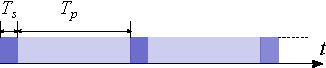
\includegraphics[scale=1]{sensing_period.pdf}
\caption{Sensing duration $T_s$ and sensing period $T_p$}
\label{fig:sensing_period}
\end{figure}



The sensing duration $T_s$ includes both detection time in physical layer and the decision synchronisation time.
Sensing period $T_p$ is the time between two successive sensing durations.
If the channel is sensed as busy\footnote{Concrete sensing techniques are not discussed in this chapter.} in sensing duration, which means at least one primary user in the vicinity is in ON state, we say the state of primary user is labelled as ON in the following sensing period $T_p$.
If not a single primary user is sensed, primary users in vicinity in the following sensing period is said to be in state OFF.
Secondary user senses each licensed channel for time $T_{access}$ with round robin scheduling, and records statistics of ON/OFF states of that channel at its place.
%In the process of transmission, as sensing is still conducted every $T_s+T_p$ time, the sensing record is updated by the sensing result in the previous $T_{access}$ time. 
%Spectrum sensing is conducted periodically, the statics on ON/OFF states are stored to update the virtual coordinate when needed.
%Such statistics are used to give quantitative spectrum availability on each node, which is further used to obtain spectrum aware virtual coordinate, besides, they are also adopted as reference to choose working channel when sending packets.


\section{Spectrum Aware Virtual Coordinates}
In this section, we firstly introduce how spectrum aware virtual coordinate is assigned, then we introduce two normalized spectrum utilities on secondary user adopted in the virtual coordinate assignment process.
One of them is called \textit{normalized spectrum availability} which is on the basis of duty cycle of primary users' absence, the other is called \textit{normalized longest blocking time} which as the name tells, is based on the lengths of time durations that primary users are detected.

Virtual coordinate has been proposed in sensor and ad hoc networks~\cite{gpsfree05infocom,Alizai_11_probabilisticAddressing}.
%Virtual coordinate is able to replace actual physical position for geographic routing in many different scenarios.
In the left part of Figure \ref{fig:vc_intro}, nodes are labelled with physical positions.
The right hand side part shows the same network assigned triplet virtual coordinate for each node according to virtual coordinate assignment protocol (\gls{VCap})~\cite{gpsfree05infocom}, where each element of the coordinate denotes the minimal number of hops away from corresponding anchor.
This kind of virtual ordinate belongs to tree based virtual coordinates, and is obtained based on anchors which locate at the edge of network.
Anchor messages are broadcast from anchors, each of them contains a counter recording the number of hops travelled.
The minimum counter of the arriving anchor messages constitutes the corresponding element of the virtual coordinate on the arrival node.
Except for the hope numbers away from certain anchor node, virtual coordinate can also be composed with link quality~\cite{Alizai_11_probabilisticAddressing} in wireless sensor networks.
The hop based virtual coordinate is independent on actual physical position, but %reflects distance and closeness of nodes on certain aspects, and can 
supports greedy geographic routing successfully \cite{gpsfree05infocom, Alizai_11_probabilisticAddressing}.
%xxxxx The euclidean distance calculated with virtual coordinate is adopted in geographic routing.
For example, when the source-destination is B and D, and Euclidean distance calculated with virtual coordinate is adopted in the routing decision, then the greedy geographic routing achieves the same routing path in both networks: $B\rightarrow C\rightarrow D$. This path is one with the shortest traversal distance.


\begin{figure}
\centering
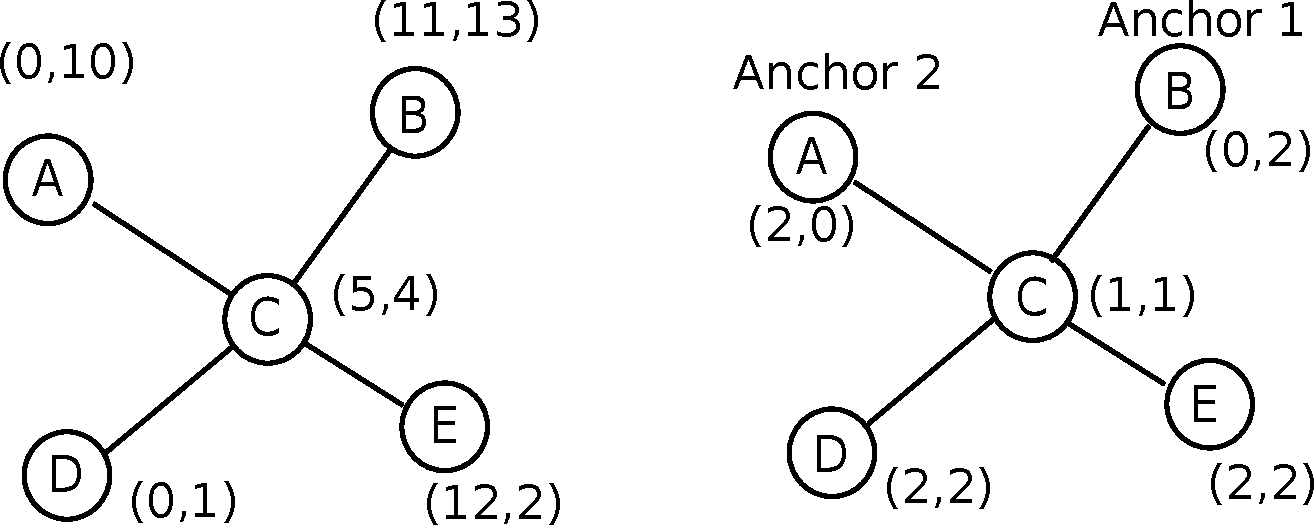
\includegraphics[scale=0.5]{vc_intro.pdf}
\caption{Left: nodes with physical locations, Right: nodes with doublet virtual coordinate, each element in the virtual coordinate is the number of hops away from corresponding anchor. Connecting lines denote the communication is possible.}
\label{fig:vc_intro}
\end{figure}


In this chapter, we propose licensed spectrum aware virtual coordinate in CRN, which enables geographic routing to find the path with better available spectrum.
%First of all we briefly introduce the virtual coordinates assignment protocol (VCap)~\cite{gpsfree05infocom} which is designed for wireless sensor networks working with unlicensed spectrum band.
Figure~\ref{fig:SA-VCapidea} shows one CRN where secondary users are assigned virtual coordinate according to anchor 1.
The transmission opportunity of the nodes locating within primary users' transmission range, \eg node A and C, is decreased due to sporadic spectrum, as a result, the cost for packet transmission, \eg transmission delay and energy consumption, is increased.
We integrate this obstacle caused by spectrum scarcity to transmission into virtual coordinate.
%When the anchor message arrives at node D, the counter add itself with a quantified value representing the spectrum availability, and the new value of the counter becomes the virtual coordinate of the arrival node.
%For example, as node A and C are influenced by primary users, the quantified spectrum availability on them is 3 and 4, on the other hand, quantified spectrum on node B, E, D is 1. 
%When we apply the anchor spreading as defined by VCap, and replace hop with quantified spectrum availability, we obtain the virtual coordinate for each node as Figure~\ref{fig:SA-VCapidea} shows.
%The definition of quantified spectrum is introduced in section~\ref{CA_VC_likelihood} and \ref{BT}.


%Obviously, how to characterize the channel availability (or equivalently, PU's influences) with link length is critical for the design of spectrum aware VC.
\begin{figure}
\centering
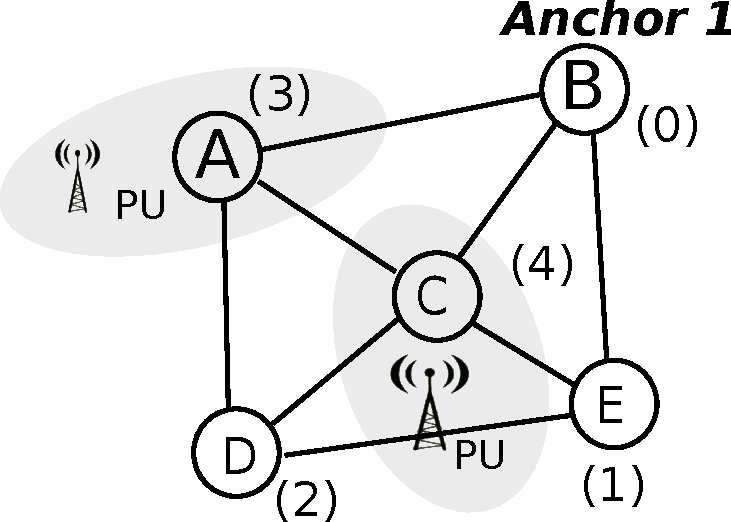
\includegraphics[scale=0.5]{CAVCap_idea_paper.pdf}
\caption{A network under primary users' influence assigned with SAViC, only anchor 1 is adopted. Flooding of anchor messages is not shown.}
\label{fig:SA-VCapidea}
\end{figure}


\subsection{Assign Spectrum Aware Virtual Coordinate}

%Similar with VCap~\cite{gpsfree05infocom}, SAViC consists of four rounds of anchor message flooding initiated from four anchors $A$, $X$, $Y$, $Z$ respectively.
As to SAViC, anchors broadcast anchor messages which flood over the network and result in virtual coordinate for each secondary user.
Several anchors are needed to assign unique virtual coordinate for each secondary user.
How to select anchors is out of the scope of this chapter.
%Each round of anchor message flooding results in one value on each node, and the last three values $x$, $y$, $z$ compose the triplet of virtual coordinate $\{x,y,z\}$.
%Besides, each node also has one auxiliary quadruplet virtual coordinate $\{a',x',y',z'\}$ which is used to decide on anchors.
In the following, we introduce how is virtual coordinate decided on each node with respect to anchors.
%Each coordinate is composed with four elements which correspond to four anchors $A$, $X$, $Y$, $Z$ respectively.


Each secondary user maintains its virtual coordinate which is one $r$-tuple where each element contained corresponds to one anchor, and the tuple length is $r$.
The elements of virtual coordinate on each node is set as big positive value.
An anchor message is generated on the anchor, which contains a $counter$ whose value is set as 0.
The anchor message is broadcast on control channel.
The influence of primary users on a secondary user is quantified as spectrum utility $\lambda$ on that secondary user.
The bigger value indicates heavier spectrum occupation by primary users.
$\lambda$ will be discussed in Section~\ref{CA_VC_likelihood} and \ref{BT}.

When a node $i$ receives an anchor message from the $t$th anchor, $i$ compares the $t$th element in its current virtual coordinate with the sum of the $\lambda$ and $counter1$ which is contained in the arriving anchor message.
%When a secondary user receives anchor message originating from anchor $A$, it adds the normalized channel availability $\Psi$ (introduced in next subsection) on itself and VC\_counter which is contained in the message, and compares the summation with its own $VC_i$.
If the sum is greater than the $t$th element in its current virtual coordinate, which indicates that the path traversed by this anchor message exposes to more active primary users, node $i$ drops the anchor message.
If the sum is smaller than the $t$th element in its current virtual coordinate, the node set the $t$th element as the sum and updates $counter1$ contained in the anchor message before forwarding it.
%The acquisition of auxiliary coordinate \textit{a'} is very similar with that for virtual coordinate.
This process is presented as Algorithm~\ref{algo:receiveAnchorMessage}.
% which also applies to obtain virtual coordinate and auxiliary coordinate in other rounds.
The process ceases within a period of time.
\begin{lemma}
\label{savic:lemma1}
The times that one secondary node forwards the anchor messages which are associated with one specific anchor is bounded by $g$, where $g$ is the number of one hop neighbours of that anchor.
\end{lemma}

\begin{lemma}
\label{savic:lemma2}
The counter value of one anchor message is increased after it is forwarded.
\end{lemma}
\begin{proof}
This is proved by the lines 18-20 in Algorithm~\ref{algo:receiveAnchorMessage}.
\end{proof}

\begin{lemma}
\label{savic:lemma3}
One anchor message affiliated with one anchor visits any secondary user at most twice.
\end{lemma}
\begin{proof}
Assume one node is accessed by the same anchor message for two times.
When the anchor message arrives at the secondary user, let's say $i$, for the first time, there is $\text{vc} > counter+\lambda$, and both of the vc and counter in the anchor message are updated to be $counter+\lambda$.
After being forwarded, the anchor message travels at least one other secondary user before arriving $i$, and the counter is greater than the counter value when it is forwarded from $i$ according to Lemma \ref{savic:lemma2}, which means, current counter value is greater than $\lambda_i$, and the anchor message is dropped.
Thus, this anchor message accesses secondary user $i$ for at most two times.
\end{proof}

\begin{theorem}
\label{savic:theorem_anchorMsg}
The number of anchor message corresponding to one anchor is bound by $2*g*n$, where $n$ is the number of secondary users.
\end{theorem}
\begin{proof}
This is proved by Lemma~\ref{savic:lemma1} and \ref{savic:lemma3}.
\end{proof}

According to Theorem~\ref{savic:theorem_anchorMsg}, every secondary users obtains virtual coordinate which respects to all anchors after a finite time duration.
%The algorithm for secondary user $i$ to receive one element $vc_i$ is given in Algorithm~\ref{algo:receiveAnchorMessage}.
\begin{algorithm}[!h]
\caption{Secondary user $i$ obtains one element $vc_i$ in its VC with respect to an anchor}%, $\lambda_i$ is normalized spectrum availability on $i$}          % give the algorithm a caption
\label{algo:receiveAnchorMessage} 
\DontPrintSemicolon
\SetAlgoLined
\KwIn{$vc_i =M$, $M$ is one big positive number}
%\KwOut{}
\lnl{InRes1}\If {$i$ is anchor}{
\lnl{InRes2}$vc_i=0$;\\
%\lnl{InRes3}$VC\_counter=\Psi_i$ \\ %\tcc*[f]{or $\Lambda_i$, based on }
\lnl{InRes4} set $counter1=\lambda_i$ in anchor message;\\
\lnl{InRes5} broadcast anchor message;\\
}

\lnl{InRes6}\If{receive anchor message}{
\lnl{InRes7}\eIf{$counter +\lambda_i \geqslant vc_i$}{
\lnl{InRes8}drop anchor message;}{
%\lnl{InRes9}$VC\_counter + \Psi_i < VC_i$  \\
\lnl{InRes9}$vc_i=counter + \lambda_i$;\\
\lnl{InRes10}set $counter=vc_i$ in anchor message;\\
\lnl{InRes11}broadcast anchor message;
}
}
\end{algorithm}


% which previously was stable at a low level during a long period of time. 



%and the two resultant virtual coordinates, duty cycle based virtual coordinate and blocking time based virtual coordinate.
%They are used to construct virtual coordinates which are tailored for different applications, i.e. file transmission which requires higher PDR, or instant communication which demands small end to end delay.
%virtual coordinate Dissemination


\subsection{Normalized Spectrum Availability on Secondary Users}\label{CA_VC_likelihood}
Based on the statistics of primary user's ON/OFF states in time duration $T_{assement}$ which contains multiple $T_s$, secondary user $i$ characterizes the likelihood that one licensed channel, say $k$, is available at its own position with \textit{duty cycle}, which is
\begin{equation}
\label{gamma}
\gamma_i^k = \frac{\Delta_{\textsc{\tiny OFF}}}{\Delta_{\textsc{\tiny OFF}}+\Delta_{\textsc{\tiny ON}}},
\end{equation}

%\begin{equation}
%\label{likelihood_channel}
%\begin{aligned}
%\gamma_i^k = \frac{\Delta_{\textsc{\tiny OFF}}}{\Delta_{\textsc{\tiny OFF}}+\Delta_{\textsc{\tiny ON}}}
%\end{aligned}
%\end{equation}
where $\Delta_{\textsc{\tiny OFF}}$ is the number of sensing periods when channel $k$ is sensed as OFF in $T_{assement}$.
%$\gamma_i^k$ represents the likelihood that $i$ is allowed to access the licensed channel $k$.
To implement SAViC whose resultant Euclidean distance between two nodes reflects both influence from primary users and distance in terms of hops, we need to design a normalized quantified spectrum availability $\lambda_i$.

\subsubsection{Single licensed channel}
When there is only one licensed channel in CRN (the superscript of channel $\lambda$ is omitted), the normalized spectrum availability on node $i$ is proposed as,% (upper script for channel is omitted for clarity), 
\begin{equation}
\lambda_i = -\ln \gamma_i+ c \cdot \gamma_i
\label{singCH_onehop_dc_metric}
\end{equation}

%As $\gamma_i$ denotes the possibility that one CR can deal with on packet at one time, for the path composed with series of CR nodes, the possibility that the packet travels through the path without going to buffer due to primary users occupying channel is the product of $\gamma_i$ on all nodes along the path.
%The virtual coordinate obtained by Algorithm~\ref{algo:receiveAnchorMessage} and equation~\ref{singCH_onehop_dc_metric} and 
With Formula \ref{singCH_onehop_dc_metric}, when one anchor message which originates from anchor $X$ is forwarded from node $a$ to $b$ without being dropped, the distance based on virtual coordinate reflects both the spectrum availability and geographic distance in terms of hops between the two nodes.
Based on Algorithm~\ref{algo:receiveAnchorMessage} and Formula~\ref{singCH_onehop_dc_metric}, the distance in dimension X is, 
\begin{equation}\label{distance}
\begin{split}
|x_b-x_a| & =  \sum_{i\in P_{(a,b]}} (-\ln\gamma_i + c\cdot \gamma_i) \\
		  & = -\ln(\prod_{i\in P_{(a,b]}} \gamma_i) + c\cdot \sum_{i\in P_{(a,b]}} \gamma_i
\end{split}
\end{equation}
here $x_a$ and $x_b$ are virtual coordinates of node $a$ and $b$ in dimension X respectively.
$P_{(a,b]}=(\cdots, b)$ denotes the list of nodes after $a$ and till $b$, which forward the same anchor message.

The reason to choose the form of Formula~\ref{singCH_onehop_dc_metric} is as follows.
As Formula~\ref{distance} shows, the first item is logarithm of the product of consecutive spectrum availability likelihood of the nodes in $P_{(a,b]}$.
The product is the likelihood that one message travels from node $a$ to $b$ without hampered by primary users, which is an important property we want to integrated into our virtual coordinate system.
The fist item will be infinity when the spectrum is occupied by primary users during all the time, where $\gamma=0$.
In this case, infinity can be replaced with a large positive value which results in a large $\lambda$.
The second item denotes number of hops, which can be seen clearly when $\gamma_i=0$ for node $i\in P_{(a,b]}$.

As $\lambda_i$ needs to be monotonically decreasing with respect to $\gamma_i$, so that the less spectrum availability results in bigger cost for communication, thus there should be
\begin{equation}
\frac{\partial\lambda_i}{\partial\gamma_i} = c -\frac{1}{\gamma_i} <0
\label{singCH_dc_metric_decreasing}
\end{equation} 
hence the tuning parameter $c$ should be smaller than 1.
In the simulation part, we choose $c=0.2$ so that $\lambda$ visibly reflects the changes of $\gamma$ when $\gamma$ is not too small, as Figure~\ref{fig:gamma_lambda} shows.

\begin{figure}
\centering
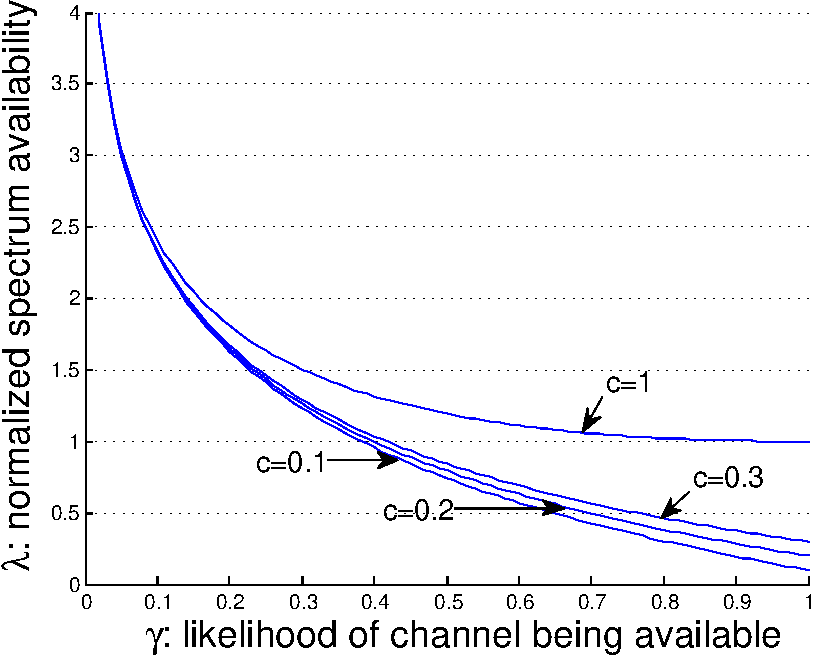
\includegraphics[scale=0.7]{gamma_lambda.pdf}
\caption{Normalized spectrum availability with respect to the likelihood of spectrum being available one a node}
\label{fig:gamma_lambda}
\end{figure}

%identical virtual coordinate not to be given when nodes locate out of primary user's transmission range.
%In that case the second item is positive (the first item becomes 0), so node receives a distinguishing virtual coordinate from the neighbour where the anchor message is sent out.
%and we can tune the coefficient c to adjust the weight of hops.

%2. If $a$ and $b$ don't have any coordinate obtained from the same anchor message, the distance between the two nodes with virtual coordinate is limited times of the real distance.
%see figure!!!

%Echoing the idea of virtual coordinate assignment in Figure \ref{fig:SA-VCapidea}, this function should be monotonically decreasing with respect to $\lambda_i$, thus the tuning parameter $c$ should be smaller than 1.ZA


\subsubsection{Multiple licensed channels}
When multiple licensed channels are allowed to use without interfering primary users, one node can switch to an another channel which is at present available to send or forward packet, then the normalized channel availability is,
\begin{equation}
\gamma_i = 1-\prod_{k=1}^{|C|} (1-\gamma_i^k)
\label{gamma_multichannel}
\end{equation} 
Based on Formula~\ref{singCH_onehop_dc_metric}, the normalized spectrum availability on node $i$ when multiple secondary channels are available is,
\begin{equation}
\label{mulCH_onehop_dc_metric}
\begin{aligned}
\lambda_i & = -\ln \gamma_i+ c \cdot \gamma_i\\
		&= -\ln(1-\prod_{k=1}^{|C|}(1-\gamma_i^k)) + c \cdot (1-\prod_{k=1}^{|C|}(1-\gamma_i^k))
\end{aligned}
\end{equation}


\subsection{Normalized Longest Blocking Time on Secondary Users}
\label{BT}
Channel utility introduced in previous subsection characterizes the likelihood that secondary user is allowed to forward packets, but it fails to reflect the availability of spectrum in a finer granularity of time.
For instance, in the period of time $T_{access}$ to access the spectrum availability, one channel which frequently changes between state ON and OFF due to primary users' violent operation may have the same likelihood of available spectrum with the channel where primary user sojourns on state ON for long time.
This difference has direct consequence on delay when the likelihood of spectrum availability on PU affected secondary nodes is homogeneous.
%As to the two circumstances, when one secondary user has packet to send but spectrum is occupied completely by primary users at that time, this node needs to wait different length of time before the spectrum becomes available again, which is fundamental to end to end delay.

Let ${T_{ON}^k}$ be the length of time period that channel $k$ is not available, there is ${T_{ON}^k} = n\cdot (T_s+T_p)$, where $n$ is the number of consecutive sensing duration that channel $k$ is sensed as busy.
${T_{ON}^k}$ is recorded within $T_{access}$, and we use $\tau^k = \overline {T_{ON}^k}$ to denote the average value of the time duration that channel $k$ is occupied by primary user, which is the maximum time period that secondary user is blocked from sending/forwarding.
%$\tau^k$ models when channel is not available, the average maximal time needed to wait before the spectrum opportunity comes back again.

\subsubsection{Single licensed channel}
In single licensed channel scenario, the normalized maximum blocking time on node $i$ is (superscript $k$ is omitted), 
\begin{equation}
\label{eq:SingleChannel_blockingtime}
\begin{aligned}
\lambda_i = f(\tau_i) = \gamma_i\cdot \tau_i + b\cdot e^{-\gamma_i\cdot \tau_i}
\end{aligned}
\end{equation}

%proposed new metric:
%\begin{equation}
%\label{eq:SingleChannelEWTLM}
%\begin{aligned}
%\lambda_i = f(\tau_i) = -\ln\gamma_i\cdot \tau_i + b\cdot e^{-\gamma_i\cdot \tau_i}
%\end{aligned}
%\end{equation}

%We multiply $\tau$ with likelihood $\gamma$ in the first item to let $\lambda$ describe channel availability more completely.
The first item is the product of blocking time and the duty cycle of available spectrum, note that we assume the duty cycle is identical for any PU affected secondary user and thus can be regarded as constant.
As to the secondary users which locate out of any primary user's transmission range, there is $\tau_i=0$, then $\lambda_i=b$, $\lambda_i$ denotes hop count in this case.
This is the reason that the second item is needed.

Same with the analysis in section~\ref{CA_VC_likelihood}, when one anchor message travels through path $P_{(a,b]}$, the distance on the corresponding coordinate dimension is the sum of the normalized longest blocking time, which is the function of the sum of maximum blocking time on the cascaded nodes on the trajectory of anchor message,

\begin{equation}
\label{distance2}
\begin{split}
|x_b-x_a| & =  \sum_{i\in P_{(a,b]}} (\gamma_i\cdot \tau_i + b\cdot e^{-\gamma_i\cdot \tau_i}) \\
		  & = \gamma_i\cdot \sum_{i\in P_{(a,b]}}\tau_i + b\cdot e^{-\gamma_i\cdot \sum_{i\in P_{(a,b]}}\tau_i}
\end{split}
\end{equation}

%As to get virtual coordinate, secondary user simply adds its normalized maximum delay onto the $counter$, so that its virtual coordinate denotes the maximum delay on the trajectory from it to anchor.

Normalized longest blocking time $\lambda$ is monotonically increasing with $\tau_i$, which requires
\begin{equation}
\begin{split}
\frac{\partial\lambda_i}{\partial\tau_i}=\gamma_i-\gamma_i\cdot b\cdot e^{-\tau_i\cdot \gamma_i}  >0\\
b  < e^{\gamma_i\cdot \tau_i}
\end{split}
\end{equation}
then we set the tuning parameter $b$ as 1.

\subsubsection{Multiple licensed channels}
In multiple licensed channel scenario, $\tau_i$ equals to the smallest maximum blocking time over all secondary channels on node $i$, 
\begin{equation}
\tau_i = \min \tau_i^x, x\in C
\end{equation}
The normalized maximum blocking time on node $i$ is as Formula~\ref{eq:SingleChannel_blockingtime} shows.

%\begin{equation}
%\label{Tau}
%\lambda_i = f(\tau_i^k) = \gamma_i^k\cdot \tau_i^k+ b\cdot e^{-\gamma_i^k\cdot \tau_i^k}, 
%\end{equation}

%and $b$ should satisfy $b < e^{\tau_i^k\cdot \gamma_i^k} $

%where $k = \underset{c}{\operatorname{argmin}} \tau^k, c\in C$.
%In a word, $\Lambda_i$ is decided by the smallest $\tau_i$ over all secondary channels.


In remainder of this chapter, the virtual coordinate based on normalized spectrum utility is referred as \textit{spectrum availability based VC}, and The virtual coordinate based on normalized maximum blocking time is denoted as \textit{blocking time based VC} out of convenience.

%\subsubsection{Distinct virtual coordinate} 
%Except for the \textit{spectrum availability} and \textit{blocking time} based virtual coordinate introduced in this section, other metrics of spectrum opportunities in CRN~\cite{spectrumDecision_2013mass} are also possible to be integrated into virtual coordinate, while, the validity of the idea of spectrum availability based virtual coordinates is not harmed.
%Due to the expressions of channel availability from Formula~\ref{singCH_onehop_dc_metric} to~\ref{Tau}, virtual coordinate is not integer but real number, thus there is little chance for nodes in a vicinity share the same coordinate.

 

%With SAViC, the size of zones where nodes are signed with identical virtual coordinate if applied with VCap is decreased, because $\lambda$ brings in the primary users' activity and alter the virtual coordinate of nodes which otherwise locates in the zone.
%To obtain virtual coordinate according to SA-VCap, each SU needs to broadcast once in each phase as is shown 
%Large amount of control messages are involved in generating VCs, but whenever 
When $\lambda$ on secondary nodes is identical, the resultant SAViC appears to be similar with hop based virtual coordinate.
In reality, as the measurement shows in \cite{measurement_Palaios14}, heterogeneity of spectrum usage by primary users is very normal, besides, the two kinds of virtual coordinates make it easier to find out such heterogeneity.
\cite{measurement_Palaios14} also shows within certain frequency band, primary users' activity is stable for hours, \eg cellular network.
When primary user's operation pattern changes, \eg occupy spectrum with increased duty cycle, then SAViC needs to be reimplemented.

\section{Geographic Routing and Opportunistic Spectrum Access}
\label{osa}
%\subsection{Improved Geographic Greedy Routing Used in Testing}
%After SAViC is applied in CRN, geographic routing is used and the routing metric is the remaining Euclidean distance to the destination. 
Although spectrum aware virtual coordinate is the main concern of this chapter, we also introduce the geographic routing to be used as it affects the routing result directly.
With geographic routing, packet sender/forwarder chooses the neighbour which has smaller Euclidean distance to the destination.
The distance between node $i$ and destination $d$ is $\sqrt{(x_d-x_i)^2+(y_d-y_i)^2+(z_d-z_i)^2}$, when virtual coordinate can be denoted as $\{x, y, z\}$.
A trivial improvement on greedy geographic routing is implemented in network layer to mitigate the dead end problem.
When routing protocol reaches dead end node $u$ which is closest to destination, $u$ adds its ID to the packet as taboo before forwarding the packet to $v$ which is closest to the destination in its neighborhood.
The packet will not be sent to the nodes whose IDs appear to be taboos.
%As to deciding working channel in multiple channel scenario, packet sender only needs to exchange message with next hop for once (will be explained in Section~\ref{osa}).

%As discussed in \cite{gpsfree05infocom}, when VCap is applied, there exists an area of nodes which have the same virtual coordinate.
%Zone of identical virtual coordinate also appears when applying SAViC, which is discussed in Section \ref{Duplicated_Virtual_Coordinate}.
%When the packet arrives at one node with the desired virtual coordinates but wrong ID, the arriving node broadcasts to look for the node with desired ID, if get replied, the packet will be sent to the desired node.





%  in its neighborhood, but from where the routing protocol can not progress towards to the destination, either because it has no other neighbour, or its neighbours have been labelled as dead end.
%When packet reaches a dead end, it attaches the node ID into the packet, and is sent back to the sender.
%The dead end list contained in the packet will help packet forwarder decide on the next hop.
%When one node has packet to send, it chooses the neighbour which is closet to the destination (even further than the sender) as next hop as long as it is not in the dead end list encapsulated in the packet.
% Face routing~\cite{routingMetric_greedyRouting09infocom} overcomes dead end problem completely, but it is not considered here because of its complexity.

Buffer is implemented on each node, where packets stay temporally when no unoccupied licensed spectrum is available.
Secondary user resends buffered packet every period of time, and drops it if there is still no available channel after trying for 10 times.
%$T_{buffer}$ equals to the smallest average time duration that channel is occupied by primary users, which is introduced in subsection \ref{BT}.





%It is known that geographical routing is possible to get stuck at dead end node which is more closer to the detonation than all its neighbours. Lots of solutions have been proposed~\cite{routingMetric_greedyRouting09infocom, vc-mobile-2007} to solve this problem, e.g. face routing. In this work on the basis of primitive geographic greedy scheme, we implement \textit{geoGreedy+} which involves simple workarounds to cope with dead end problem and loops on routing paths.
In multiple channel CRN, after one node deciding on the next hop via geographic routing, which channel to use needs to be answered.
This problem involves considerations from many aspects, such as minimizing channel switch cost~\cite{spectrumDecision_2013mass}, mitigating co-channel interferences~\cite{DySpAN12_Di} etc..
%Channel selection is an active research topic which involves interference mitigation~\cite{DySpAN12_Di}, power control~\cite{HoangPowerChannel2010}, scheduling~\cite{MOBICOM10_retransmission}, topology control~\cite{Li11_ROSS}, etc.
We adopt a lightweight heuristic method in this chapter. 
When there is packet to send and the next hop is decided, packet sender chooses the channel in descending sequence with channel's metric, i.e., likelihood of channel availability, or blocking time.
The sender chooses the channel with the best metric, then conducts spectrum sensing in the immediately following sensing duration to determine the channel's usability.
If the channel is sensed as free to use, sender transmits \textit{request\_channel\_x} to the next hop on the control channel, when it receives the answering message \textit{channel\_x\_available} from that node, it starts communication on channel $x$ in the following sensing period.
If the channel is sensed to be busy before or among the transmission, or it receives \textit{channel\_x\_unavailable} message from next hop node, the sender moves to the channel with the second best metric, and conduct the same procedure as described above.
%As to delay based SAViC, the channel access strategy is the same as above except the metric to choose channel becomes $\tau$, the average time duration of being blocked instead of $\gamma$.




\section{Performance Evaluation}
%We show performance of SAViC on two aspects via simulation.
In this section, we present the performance of geographic routing together with SAViC.
Both virtual coordinates based on metrics of spectrum availability and blocking time respectively are evaluated.
Prior to that, the set-up of simulation is introduced.


\subsection{Simulation Setup}
In this section, we introduce the deployment of the primary users to generate various spectrum availability in the network, then introduce the important parameters in simulation.
Different from \cite{gpsfree05infocom} where simulation is conducted without considering any activities in MAC and physical layer, simulation in this chapter deploys a wireless environment which is close to reality, \eg interferences and channel shadowing are involved.


\subsubsection{Primary Users}
Measurements~\cite{ProbabilityAndComputing, dsa_model_markov_2006} show that the sufficiently accurate statistic model of spectrum occupancy can be given by a Markovian process.
In simulation, primary user alternates state between ON and OFF as a two-state discrete time Markov chain (\gls{2TDMC}).
% the process of alternating states of primary user.
%Primary user changes its state between ON and OFF according to transition probability, i.e. probability that it changes from current state to the other, or stays in the same state.
The probability that it changes from one state to the other, or stays in the same state is called transition probability.
Transition probability further decides the stationary probability of 2DTMC, which represents the percentage of time that primary user is in state ON or OFF in a long run.
The relationship between stationary probability $\Pi=\{\pi_{\textsc{\tiny ON}}, \pi_{\textsc{\tiny OFF}}\}$ and duty cycle $\gamma$ is, 
\begin{equation}
\label{stationary_probability}
\lim\limits_{T_{assement} \to \infty }{\gamma} = \pi_{\textsc{\tiny OFF}}
\end{equation}
Transition probability also decides the continuous sojourning time of primary user on a certain state, which affects the longest blocking time sensed by secondary users.
%~\footnote{The computation is not shown here because of space.}. 
Hence, by adjusting transition probability, we can let primary user operate with desired intensity, i.e. stationary probability for being in state OFF, or continuous sojourning time of being on state ON.
We denote stationary probability of state OFF as $P_{\textsc{\tiny OFF}}$, and the maximal blocking time as $T$.
In the following, we only use $P_{\textsc{\tiny OFF}}$ and $T$ to define primary user's dynamics, and omit mentioning the transition probability.
The time unite of the DTMC for primary user to follow is 0.1s.

As spectrum availability based and longest blocking time based virtual coordinates are designed for CRN which is influence by certain primary user activity, we design two primary user distributions.
% certain  where a certain regional disparity of spectrum exists, i.e., the former is suitable where primary users appear at some places or their occupation on spectrum is heterogeneous in the network, whereas the latter is designed where spectrum availability is identical across the network, but due to different operation pattern of primary users, the blocking time in some areas are different from the rest of the network.
As a result, we design two categories of primary user settings to evaluate the routing performance assisted by the two categories of virtual coordinate respectively.
\begin{itemize}
\item As to spectrum availability based virtual coordinate, two primary users are located in the CRN which can not affect all the nodes in CRN, as shown in Figure~\ref{fig:singleChannelPioff_case_topo}.
\item For blocking time based virtual coordinate, network is evenly covered by primary users which have the same duty cycle, but some primary users have different blocking time with the others, as Figure~\ref{fig:multipleChannelPioff_case_topo} shows.
%In  all primary users have the same spectrum availability, but some of them have shorter sojourning time in state ON than the others.
\end{itemize}
When multiple channel scenario is to be investigated, existing primary users simply start to work with current and additional channels, and there is no new primary users appear.



\subsubsection{Parameter Setting}
Simulation is conducted with INET framework provided by OMNeT++ simulator~\cite{omnetpp_paper08}, which comprises both generation of SAViC and following geographic routing. 
Secondary users are randomly distributed in a square area and 6 nodes which locate at the edge are deployed as anchors.
%The transmission power of secondary users is 0 dBm, noise is -110 dBm, the SNR threshold is 4dB, sensitivity is -90dBm, path-loss coefficient is 2, Rayleigh fading is brought in the channel model.
%As a result, to the communication range is about 10\% of the whole network.
%Licensed channel works on 2.4 GHz frequency band.
%In each network, one source node is chosen to send UDP stream to one destination node, the packet size is 512k Byte. 
%The tuning parameters $c$ and $d$ for Formulas 1 to 4 are 0.2 and 1 respectively.
%We run each simulation for 1000s, the first 95s is for secondary users to trace spectrum availability, 5s is used assign SAViC to network, the rest 900s is for routing.
%All the confidence intervals (CI) are according to 95\% confidence level.

\subsection{Success Rate of Geographic Routing on Finding Path}

We evaluate SAViC's reachability, i.e. given the virtual coordinate of destination, geographic routing forwards packet from source to the node with the desired virtual coordinate.
%We see the routing path is set up as long as any node with the same virtual coordinate is reached, and this comparison don't involve any influence from primary users when the routing is conducted.
%, and hop based virtual coordinate gains benefit because there could exist several nodes assigned identical virtual coordinate with the destination node.
%For network assigned with CA-VCs, the PUs in the network are set to state OFF when conducting geographic routing.
The comparisons are real geographic location, and hop based virtual coordinate according to VCap~\cite{gpsfree05infocom}. 
We deploy 6 anchors and then there is no duplicated virtual coordinate among the resultant virtual coordinate system.
%We configure different spectrum availability in the network to investigate the reachability of SAViC, as shown in the following table.
% so adopting different configurations of primary user in the simulation doesn't arise question of cherry picking.
%As to testing channel utility based SAViC, two primary users locate in the middle of the network as shown in Figure~\ref{fig:singleChannelPioff_case_topo}, which operates with the same $P_{\textsc{\tiny OFF}}$.
%As to delay based SAViC, primary users locate as shown in Figure~\ref{fig:multipleChannelPioff_case_topo} where each cycle center locates one primary user,.
%Two scenarios present distinctive activity patterns of primary user.
%In scenario 1, $P_{\textsc{\tiny OFF}}=0.9$ for all primary users, $T_{\textsc{\tiny ON}}$ is 27s in region 2 (the lower-left area as shown in Figure~\ref{fig:multipleChannelPioff_case_topo}), and $T_{\textsc{\tiny ON}}$ of primary user is 0.33s in region 1 (the reset area except for region 2).
%In scenario 2, $T_{\textsc{\tiny ON}}$ of primary user is 3s in region 1, other parameters of primary user is the same with scenario 1.

%\begin{figure}
%  \begin{minipage}[c]{0.65\linewidth}
%    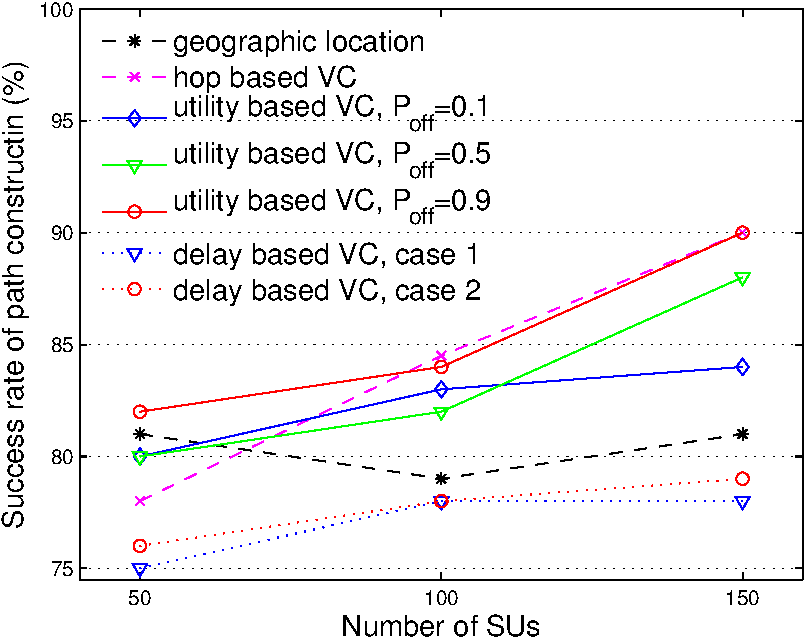
\includegraphics[width=\linewidth]{Reachability_DC_EWT.pdf}
%  \end{minipage}\hfill
%  \begin{minipage}[r]{0.32\linewidth}
%    \caption{
%			Reachability of different virtual coordinates, virtual coordinate is acronym of virtual coordinate.
%    } \label{fig:reachability}
%  \end{minipage}
%\end{figure}
%\vspace{-1cm}

\begin{figure}[ht]
	\centering
    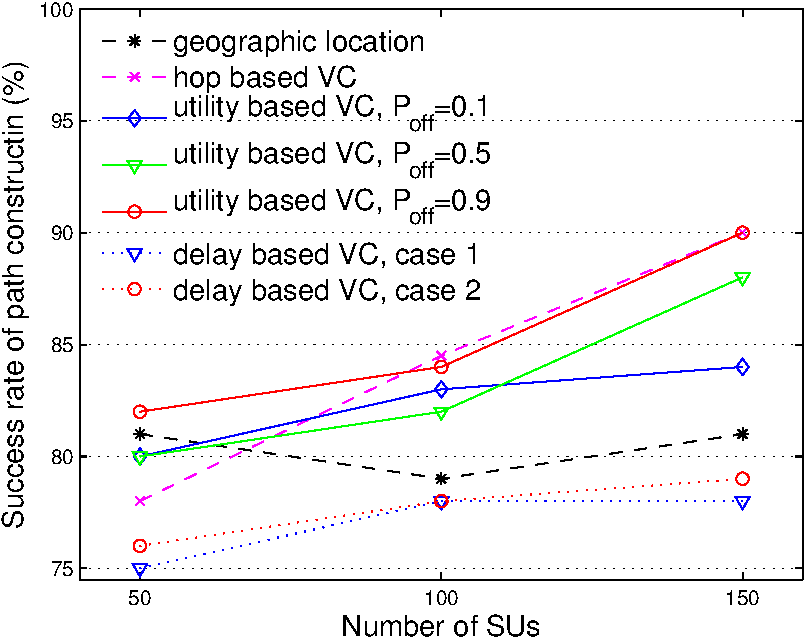
\includegraphics[width=0.7\linewidth]{Reachability_DC_EWT.pdf}
    \caption{Reachability of different virtual coordinates, the average number of neighbors is 6, 12, and 14} 			\label{fig:reachability}
\end{figure}
%\vspace{+1cm}

%There are two configurations of primary users,
%\begin{itemize}
%\item The first is as shown by the dashed cycles in Figure~\ref{fig:singleChannelPioff_case_topo}, two primary users locate in the middle of the network, which operates with the same $P_{\textsc{\tiny OFF}}$.
%This configuration is used to test Channel availability based SAViC later.
%\item The second is as shown by the cycles in Figure~\ref{fig:multipleChannelPioff_case_topo}, which is to construct one CRN where secondary users sense the same likelihood of spectrum availability, but the blocking time in some areas are different from the rest areas.
%$P_{\textsc{\tiny OFF}}=0.9$ for all primary users, $T_{\textsc{\tiny ON}}$ is 27s for primary users in solid cycles.
%This configuration is used to test Blocking time based SAViC.
%\end{itemize}
%%\vspace{-\baselineskip}
%\begin{center}
%    \begin{tabular}{| p{1.85 cm} | p{6.7 cm} |}
%    \hline
%    Coordinate & Configuration of primary users  \\ \hline
%    Channel availability based SAViC & As shown by the dashed cycles in Figure~\ref{fig:singleChannelPioff_case_topo}, two primary users locate in the middle of the network, which operates with the same $P_{\textsc{\tiny OFF}}$.  \\ \hline
%    Blocking time based SAViC & As shown by the cycles in Figure~\ref{fig:multipleChannelPioff_case_topo}, $P_{\textsc{\tiny OFF}}=0.9$ for all primary users, $T_{\textsc{\tiny ON}}$ is 27s for primary users in solid cycles
%    \vspace*{-.4em}
%\begin{itemize}%[noitemsep,nolistsep]
%  \item scenario 1: $T_{\textsc{\tiny ON}}$ is 0.33s in dashed cycles
%  \item scenario 2: $T_{\textsc{\tiny ON}}$ is 3s in dashed cycles
%\end{itemize}
%\vspace*{-1.2 em}
%      \\ \hline
%    VCap & No primary users \\ \hline
%    Geo-location & No primary users \\ \hline
%    \end{tabular}
%\end{center}

In order to evaluate the effectiveness of coordinates to support geographic routing, we design different configurations of primary users.
As to duty cycle based VC, two primary users are randomly deployed in the network.
As to delay based VC, we configure 9 primary users to evenly cover the network, among of them, 4 primary users have different maximal blocking time with the rest.
Under one configuration of primary users, 1000 random CRN is generated and in each CRN one far departed pair of source and destination is chosen to test.

%For each setting of primary user, simulation is done over 100 random secondary user networks, and in each network one pair of nodes locating at opposite ends of network (which have the largest distance) is chosen as source and destination.
%We configure two scenarios to test blocking time based virtual coordinate, scenario I: $T_{\textsc{\tiny ON}}=27s$ for the primary users in solid cycle in Figure~\ref{fig:multipleChannelPioff_case_topo}, 3s for the rest, scenario II: $T_{\textsc{\tiny ON}}=27s$ in region 2, 0.33s for the rest.

%Figure \ref{fig:reachability} depicts the average success rate of path construction of the network with the same scale.
Figure \ref{fig:reachability} shows, spectrum availability based virtual coordinate supports geographic routing to achieve similar reachability with hop based virtual coordinate\footnote{The numerical result of hop based virtual coordinate coincides with the simulation result presented in \cite{gpsfree05infocom} under the same network density}, which is better than that with real geographic location.
%When $P_{\textsc{\tiny OFF}}$ is smaller, utility based virtual coordinate works worse but the gap with the aforementioned is trivial.
%Geographic routing working with real geographic location performs poorer, because dead end problem is largely alleviated by VC.
Blocking time based virtual coordinate performs a little bit worse than other coordinates.
%delay based VC's effectiveness is illustrated in Subsection~\ref{subsection:SA-VCap-EWT} where utility based virtual coordinate fails to support geographic routing as PUs' likelihood are geographically homogeneous over the network.
%The success rate of geographic routing with hop based virtual coordinate coincides with the results in work~\cite{gpsfree05infocom}.
%Note the CRN in simulation is quite sparse compared with that used in~\cite{gpsfree05infocom}
In summary, after integrating the primary user's influence, SAViC supports geographic routing to achieve comparable success rate of path construction with conventional virtual coordinate and real geographic location.



\subsection{Routing Performance}
%%%%%%%%%%%%%%%%%%%%%%%%%%%%%%%%%%%%%%%%%%%%%%
%	single channel, channel utility based VC
%%%%%%%%%%%%%%%%%%%%%%%%%%%%%%%%%%%%%%%%%%%%%%
We sequentially present the routing performance of SAViC based on spectrum availability and blocking time respectively.
In more details, spectrum availability SAViC is compared with hop based virtual coordinate VCap and \textit{SEARCH}.
%Hop based virtual coordinate is testified to support geographic routing in large scale sensor networks successfully~\cite{gpsfree05infocom}.
The reason to choose \textit{SEARCH}~\cite{search_geo_routing_chowdhury} is it is on the basis of geographic routing and utilizes routing table in the interval of updates, thus it requires less computation ability and overhead exchanges.
%When one primary user which locates on the routing path changes its state from OFF to ON, that routing path is blocked, thus source node needs to periodically launch route request to update the possibly invalid path. 
The time interval for \textit{SEARCH} to update routing tables of the nodes on routing path is 5s.
%, and its effectiveness when channel utility SAViC becomes invalid in the case that  
%For this purpose, we use end to end delay as metric in addition to packet delivery ratio performance to give more insights into the working mechanism of virtual coordinate.
%We sequentially simulate the routing performance of SAViC based on channel utility and delay respectively, 
Both single and multiple licensed channel scenarios are investigated for the three solutions.

\subsubsection{Duty Cycle Based Virtual Coordinate} \mbox{}

%\vspace{.1cm}
%\textbf{Single secondary channel scenario}

%\textit{1. Single secondary channel scenario}
We start by looking into the performance of SAViC in single channel scenario.

%\begin{figure}
%\centering
%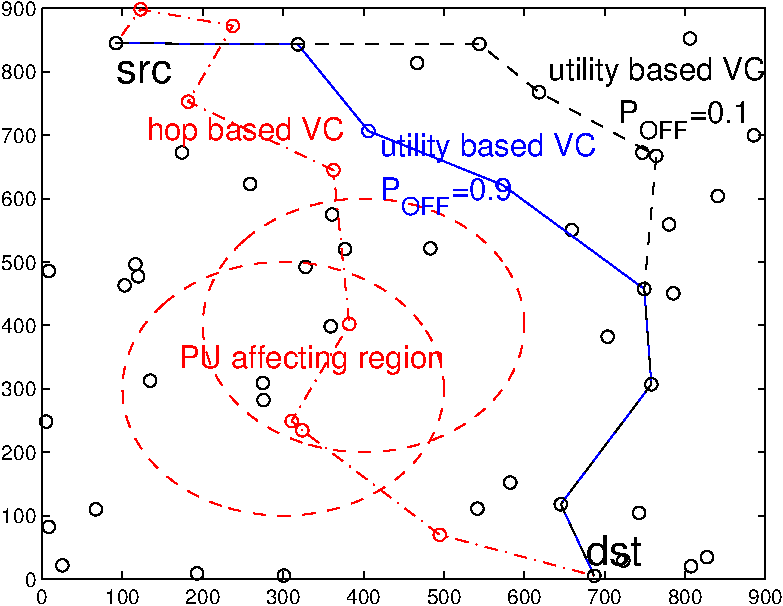
\includegraphics[width=0.5\linewidth]{singleChannel_DC_caseStudy.pdf}
%\caption{Routing paths with different virtual coordinate paradigms}
%\label{fig:singleChannelPioff_case_topo}
%\end{figure}

%\begin{figure}[htb!]
%  \begin{minipage}[c]{0.5\linewidth}
%    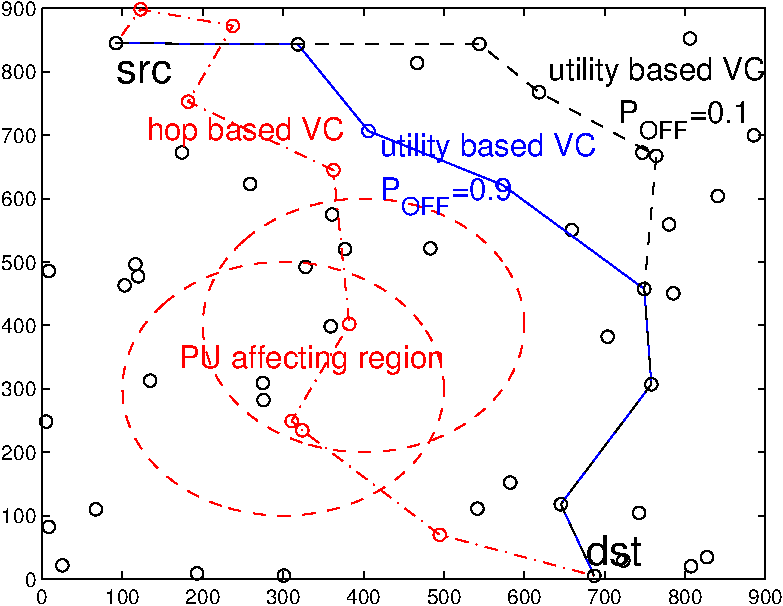
\includegraphics[width=\linewidth]{singleChannel_DC_caseStudy.pdf}
%  \end{minipage}\hfill
%  \begin{minipage}[r]{0.45\linewidth}
%    \caption{
%		Routing paths with different virtual coordinate paradigms
%    } \label{fig:singleChannelPioff_case_topo}
%  \end{minipage}
%\end{figure}


\begin{figure}[htb!]
\subfigure[Routing paths]
{\label{fig:singleChannelPioff_case_topo}
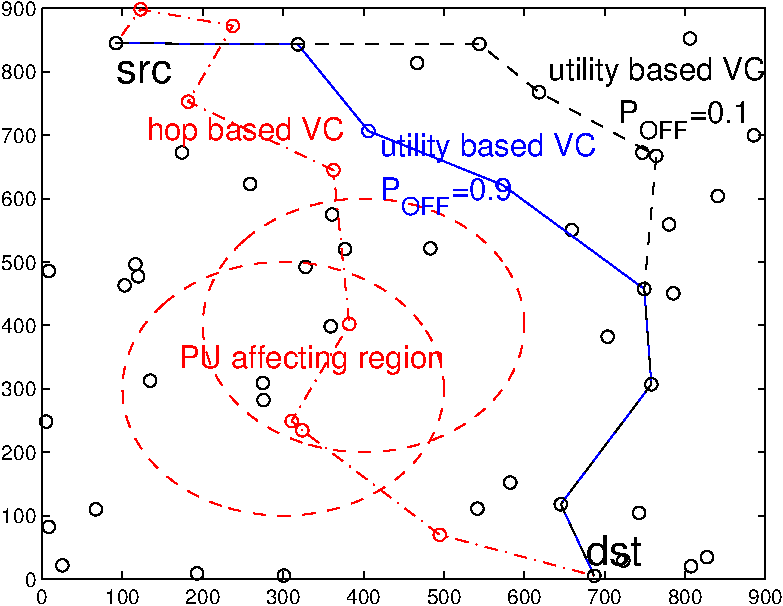
\includegraphics[width=0.455\linewidth]{singleChannel_DC_caseStudy.pdf}
}
\subfigure[PDR over 50 random CRN network, PU's location is fixed as shown in Figure~\ref{fig:singleChannelPioff_case_topo}]
{\label{fig:Averaged_single_DC}
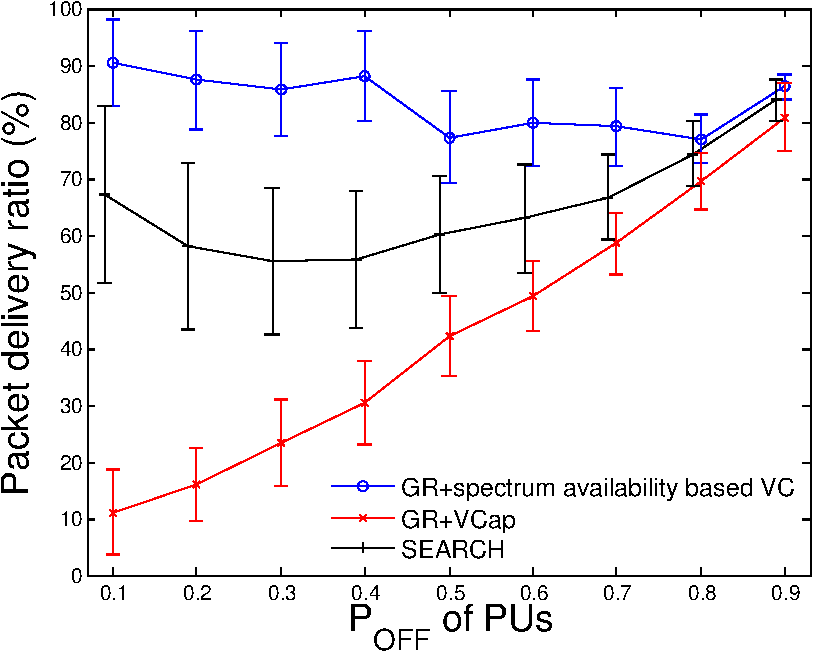
\includegraphics[width=0.455\linewidth]{singleCh_average_pdr_3.pdf}
}
\caption{Routing paths and corresponding PDR}
\label{fig:pioff_case}
\end{figure}

\begin{figure}[htb!]
\subfigure[PDR]
{\label{fig:random_SU_PU_PDR}
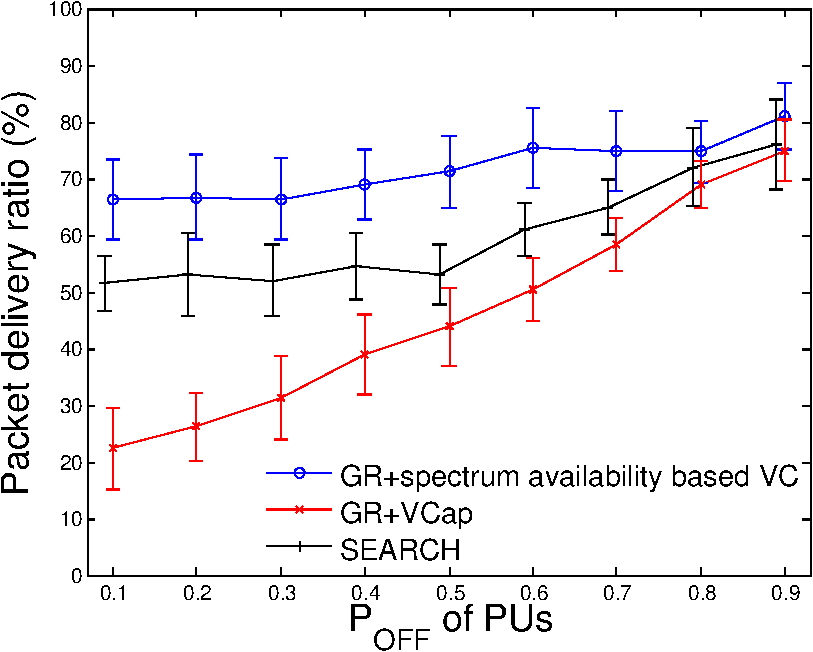
\includegraphics[width=0.455\linewidth]{random_SU_PU.pdf}
}
\subfigure[Delay]
{\label{fig:random_SU_PU_delay}
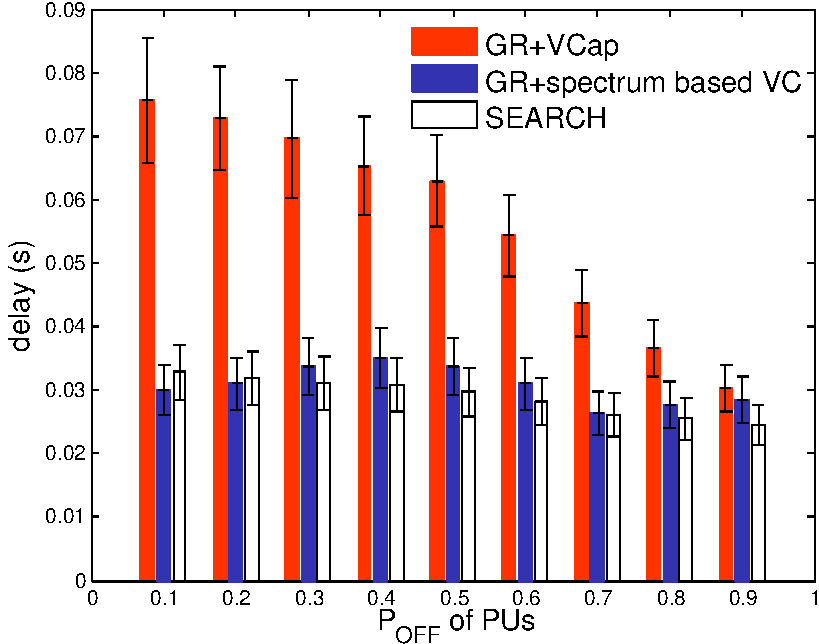
\includegraphics[width=0.455\linewidth]{delay_dc_c1.pdf}
}
\caption{Packet delivery ratio with single secondary channel, over 50 randomly located CR nodes and PUs}
\label{fig:pioff_single}
\end{figure}
We start with a case study, two primary users locate at the centers of dashed cycles as shown in Figure~\ref{fig:singleChannelPioff_case_topo}.
VC based on spectrum availability and VCap (hop is its metric) are assigned to secondary users separately.
The red dashed path in Figure~\ref{fig:singleChannelPioff_case_topo} is formed by geographic routing with VCap, which cuts across the primary users' affecting area and thus suffers great packet loss.
%The routing paths supported by spectrum availability based virtual coordinate is affected by the intensity of primary users, 
The black dash and blue solid paths are formed with spectrum availability based virtual coordinate, the two paths are formed when primary user's working intensities $P_{\textsc{\tiny OFF}}$ is 0.1 and 0.9 respectively. 
%snapshot of routing paths obtained by geographic routing with utility based virtual coordinate and hop based virtual coordinate respectively.
%When PUs' $P_{\textsc{\tiny OFF}}=0.1$, routing paths with corresponding utility based virtual coordinate is presented by the green dash line.
%Blue solid line denotes the routing path when $P_{\textsc{\tiny OFF}}$ is 0.9.
%It is easy to find that, when PUs are very active ($P_{\textsc{\tiny OFF}}=0.1$), the generated routing path detours the PU affected area completely, which means when calculated with DC-based VC, the distances between the nodes inside and outside of the PU affected area become larger, thus \textit{geoGreedy+} doesn't choose the PU affected SUs.
%When $P_{\textsc{\tiny OFF}}=0.9$, obtained routing path is closer to the PU affected areas, but is still out of the PU region.
These two paths vividly illustrate that utility based virtual coordinate successfully integrates the spectrum scarcity in CRN network, and decomposes a large part of routing decision.
%Packet delivery ratio corresponding to this network is shown in Figure \ref{fig:Averaged_single_DC}.
%Subfigure \ref{fig:SingleChannelPioff_case_pdr} presents the channel utility based VCs generate paths which achieve almost 100 \% packets delivery ratio when PU's $P_{\textsc{\tiny OFF}}$ changes from 0.1 to 0.9 in this topology.
%
%Now we step further to check channel utility based VC's ability to support geographical routing in 50 random secondary networks under different PU active levels. 
%To get full picture of SAViC's performance on packet delivery ratio, we change primary user' intensity, and randomize secondary users' location.
%We compare SAViC, hop based virtual coordinate along with one CRN routing scheme \textit{SEARCH}~\cite{search_geo_routing_chowdhury}.
The paths of SEARCH is not drawn here as the routing path is possible to change after path update.
We keep the primary users in the middle of the network, for each activity intensity, 50 CRNs where secondary users are randomly located are generated.
Figure~\ref{fig:Averaged_single_DC} shows the PDR of spectrum availability based virtual coordinate is high except for a minor decline when $P_{\textsc{\tiny OFF}}$ is between 0.5 and 0.8, which is contradictory to the monotonically increasing trend of hop based virtual coordinate. This can be explained by the path snapshot in Figure \ref{fig:singleChannelPioff_case_topo}. 
When channel is sensed to be scarce (primary users access channel intensively), path generated is far away from the affected area and circumvents completely.
When primary users become less intensive, routing path moves closer to that area.
In other words, the weaker dynamics of primary users attracts path and result in packet drop.
When $P_{\textsc{\tiny OFF}}$ approaches to 1, spectrum availability based virtual coordinate becomes actual hop based virtual coordinate as the link metric in formula \ref{singCH_onehop_dc_metric} becomes zero.
%The curve of VCap monotonically increase when PUs become less active, but it suffers seriously when PUs are active.
%The detour phenomenon of paths with utility based virtual coordinate can also be observed in Figure~\ref{fig:singleCh_DC_number_of_hops}, where route length becomes shorter when PU becomes less intensive.
%The routing paths supported by this two VCs and corresponding PDR performances are identical.
%the first item of the link metric in formula \ref{singCH_onehop_dc_metric} becomes 0 and hop metric becomes one constant, thus the paths and PDR performance generated by the two virtual coordinate systems are identical.

\textit{The paradox that more licensed spectrum leads to worse PDR} can also be observed on \textit{SEARCH}, whose PDR curve declines first and increases later on.
When channel is heavily utilized by primary users, the routing request is more likely to encounter operating primary user, then a node out of the primary user affecting area is chosen as next hop, so that the path experiences less packet loss (with the price of more hops).
When primary users become less intense, routing request is more likely to traverse the affected areas, as a result, the routing path experiences packet loss due to the primary users in that area before next route update. 
%PDR gets higher with increase of $P_{\textsc{\tiny OFF}}$ only after $P_{\textsc{\tiny OFF}}$ is bigger than 0.4.
%This is the reason for the drop of PDR in the middle
%When $P_{\textsc{\tiny OFF}}$ is bigger than 0.4, PDR gets higher with $P_{\textsc{\tiny OFF}}$ increases.
%As \textit{SEARCH} is based on geographic routing and works with real geographic location. The hop counts of routing path is shorter than that of SAViC and hop based virtual coordinate, as shown in Figure~\ref{fig:singleCh_DC_number_of_hops}.
%meanwhile, with PUs become less intense, the hop counts become smaller, which coincides with Figure \ref{fig:singleChannelPioff_case_topo}.

Figure~\ref{fig:random_SU_PU_PDR} shows the PDR when both primary and secondary users' locations are random.
SAViC's performance deteriorates because the source and destination may be influenced by primary users, so that a path completely detour the primary users' area is impossible. where geographic routing has no means to detour the affected areas.
In figure~\ref{fig:random_SU_PU_delay}, SAViC and SEARCH achieve lower delay although forwarding more packets, which means SAViC is effective to facilitate geographic routing to avoid PU affecting areas.


%%%%%%%%%%%%%%%%%%%%%%%%%%%%%%%%%%%%%%%%%%%%%%
%	multiple channel, channel utility based VC
%%%%%%%%%%%%%%%%%%%%%%%%%%%%%%%%%%%%%%%%%%%%%%
%\vspace{.1cm}
%\textbf{Multiple secondary channel scenario}
%\textit{2. Multiple secondary channel scenario}

%Formula~\ref{singCH_onehop_dc_metric} to~\ref{Tau} tell that the \textit{virtual distance} is monotonically increasing with the scarcity of spectrum, as SAViC has been testified to comprise routing decisions in CRN in previous simulation, we can firmly predict that SAViC based on Formulas~\ref{mulCH_onehop_dc_metric} to~\ref{Tau} also have similar out-performances with the same primary user setting.
%In the following, we create more challenging primary setting with more primary users.

%\begin{figure}[htb!]
%\centering
%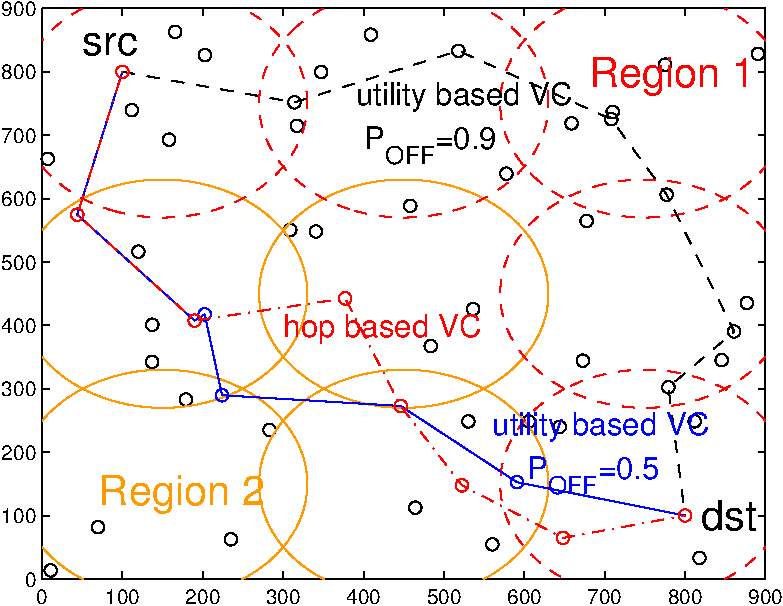
\includegraphics[width=0.5\linewidth]{MultiCH_DC_casestudy_route.pdf}
%\caption{Routing paths with different virtual coordinate paradigms}
%\label{fig:multipleChannelPioff_case_topo}
%\end{figure}

%\begin{figure}[htb!]
%  \begin{minipage}[r]{0.5\linewidth}
%    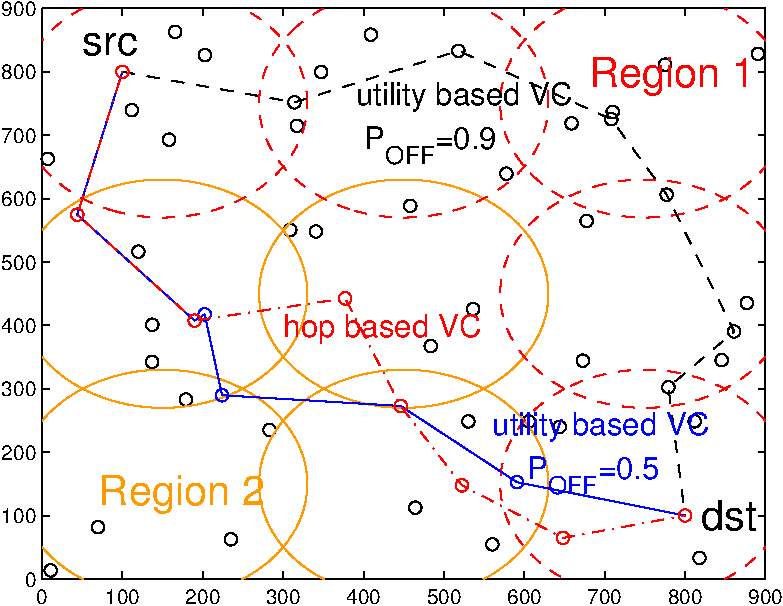
\includegraphics[width=\linewidth]{MultiCH_DC_casestudy_route.pdf}
%  \end{minipage}\hfill
%  \begin{minipage}[r]{0.45\linewidth}
%    \caption{
%		Routing paths with different virtual coordinate paradigms
%    } \label{fig:multipleChannelPioff_case_topo}
%  \end{minipage}
%\end{figure}


%\begin{figure}[htb!]
%\subfigure[One CRN]{\label{fig:multipleChannelPioff_case_topo}
%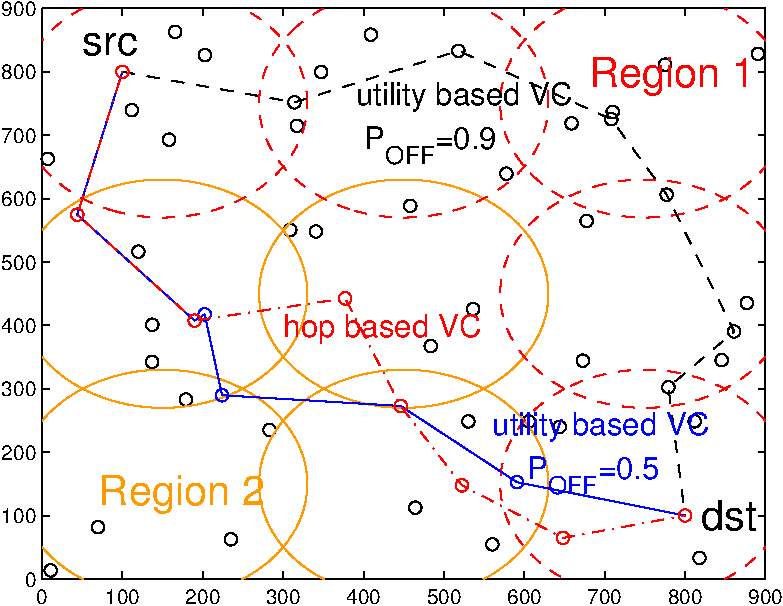
\includegraphics[width=0.455\linewidth]{MultiCH_DC_casestudy_route.pdf}
%}
%\subfigure[One CRN]{\label{fig:multipleChannelPioff_case_pdr}
%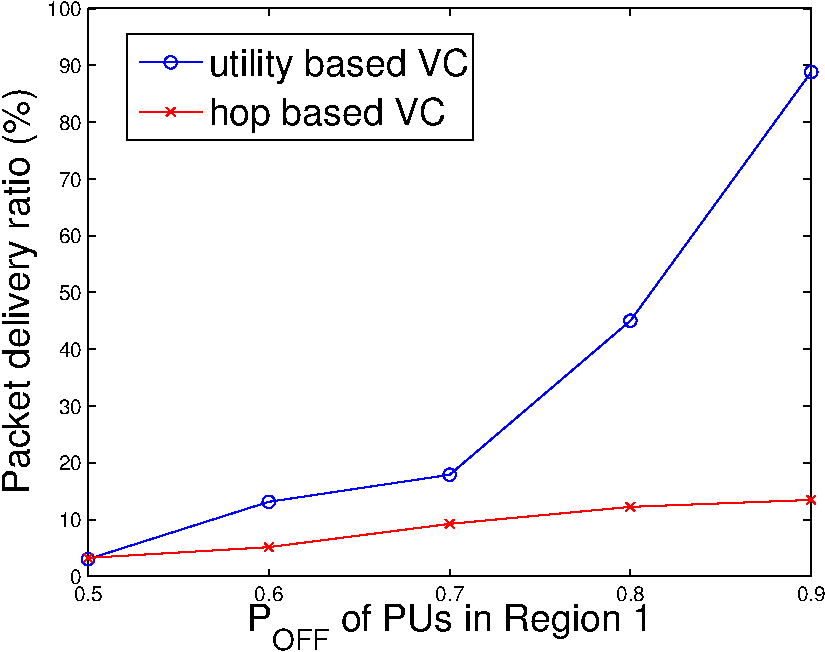
\includegraphics[width=0.455\linewidth]{MultiCH_DC_casestudy_pdr.pdf}
%}
%\label{fig:multiple_pioffCase}
%\caption{Packet delivery ratio in multiple secondary channel scenario}
%\end{figure}
Now we introduce the routing performance in multiple channel scenario, where two licensed channels available, but only one is allowed for payload transmission.


\begin{figure}[htb!]
\subfigure[PDR over 50 CRNs where SUs and PUs are randomly located]{\label{fig:MultiChannel_DC_pdr}
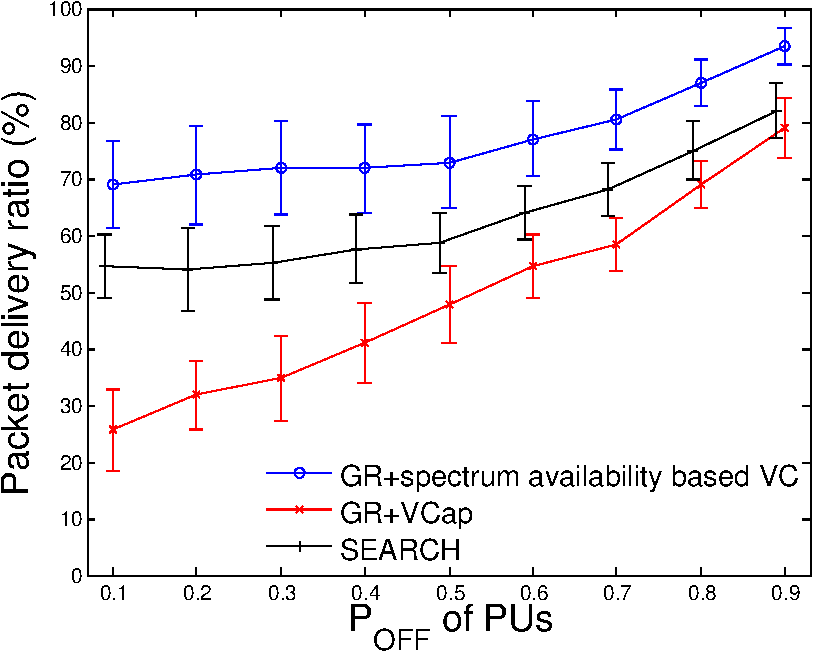
\includegraphics[width=0.455\linewidth]{random_SU_PU_2channel.pdf}
}
\subfigure[PDR over 50 CRNs where SUs and PUs are randomly located]{\label{fig:MultiChannel_DC_delay}
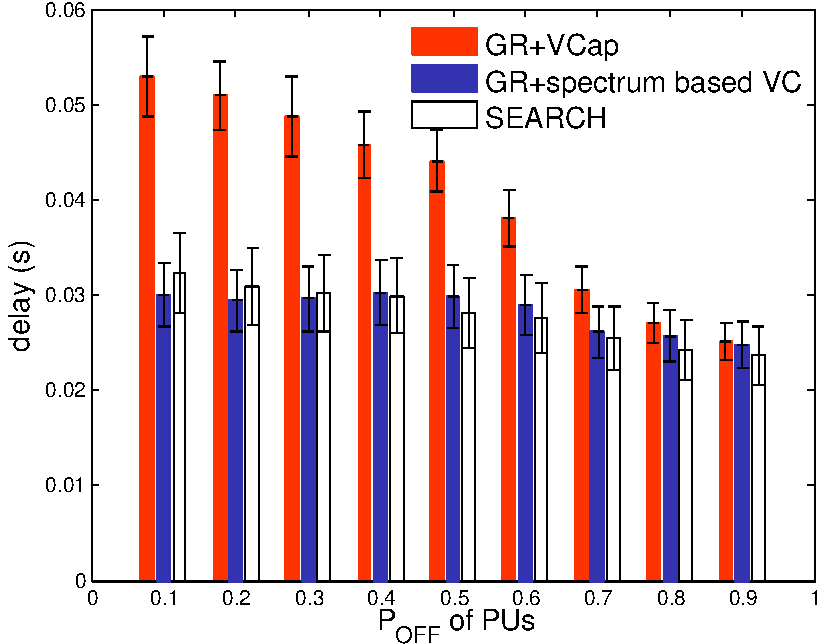
\includegraphics[width=0.455\linewidth]{delay_dc_c2.pdf}
}
\label{fig:multiple_pioffCase}
\caption{Packet delivery ratio with multiple secondary channel scenario}
\end{figure}
In this part of simulation, we follow the setting of single channel scenario, except that secondary users have at most two licensed channels.
%Network with two licensed channels is shown in Figure~\ref{fig:multipleChannelPioff_case_topo}, where primary user locates at the center of each cycle.
%Each primary user works on two licensed channels which are independent with each other.
%Figure~\ref{fig:multipleChannelPioff_case_topo} shows routing paths with different virtual coordinates and primary user's intensities, where in region 2 primary user's $P_{\textsc{\tiny OFF}}$ is 0.5.
%When $P_{\textsc{\tiny OFF}}$ is also 0.5 for primary users in region 1 and all primary users have equal workload, the path generated (blue solid path) converges to the path with hop based virtual coordinate (red dashed path).
%When $P_{\textsc{\tiny OFF}}=0.9$ for primary users in region 1, channel utility based SAViC results in black dashed path which avoids the seriously affected area.
%In this case, both paths endure tremendous packet loss as shown in Figure \ref{fig:multipleChannelPioff_case_pdr}. 
%Figure~\ref{fig:multipleChannelPioff_case_pdr} shows the packet delivery ratio of the dashed black and solid blue paths.

%Figure \ref{fig:multipleChannelPioff_case_pdr} presents the PDR of the paths generated with the two VCs.
%Most of the unsuccessfully delivered packets are dropped from buffers because of the lack of usable spectrum for too long time.
Thanks to the second channel, the packet delivery radio is increased as shown in Figure~\ref{fig:MultiChannel_DC_pdr}, and delay is decreased as depicted in Figure~\ref{fig:singleChannelPioff_case_topo}.
SAViC still outperform the other schemes especially in the aspect of PDR.
%Figure~\ref{fig:MultiChannel_DC_pdr} shows the average packet delivery ratio over 50 random topologies of secondary networks, with the same configuration of primary user as that in  Figure~\ref{fig:singleChannelPioff_case_topo}.
%Due to the second available channel and the opportunistic spectrum access paradigm, the PDR of the three schemes are improved.
%Improvement brought in by the second channel can also be observed in Figure~\ref{fig:MultiChannel_DC_delay} compared with Figure~\ref{fig:random_SU_PU}.
%Packet delivery ratio of SAViC increases with primary users become less intense, the packet loss is due to the widespread primary users.
%\textit{SEARCH} performs as bad as geographic routing with hop based virtual coordinate. The reason is the widespread primary users seriously hamper the routing requests to arrive at destination, consequentially most paths for forwarding the packets can not be constructed successfully.
%Figure~\ref{fig:MultiChannel_DC_hop} illustrates a similar trend with Figure \ref{fig:singleCh_DC_number_of_hops}, when there is less differences among PUs' intensity, the length of path becomes longer.






\subsubsection{Longest Blocking time Based Virtual Coordinate}    \mbox{}
\label{subsection:blocking_time}
%As we have pointed out in \ref{BT}, the duty cycle of channel's availability is not adequate to describe the waiting time in buffer for a packet if there is no spectrum available, thus we test the delay based virtual coordinate when all PUs' duty cycles are identical.

%This means that when primary users' certain characteristic is observed homogeneous across network, the virtual coordinate which is designed on the basis of that characteristic is not capable to comprise routing decisions any more.
%In this case another different characteristic (delay in this case) is needed to form spectrum aware virtual coordinate.

%%%%%%%%%%%%%%%%%%%%%%%%%%%%%%%%%%%%%%%%%%%%%%
%	delay based VC
%%%%%%%%%%%%%%%%%%%%%%%%%%%%%%%%%%%%%%%%%%%%%%

%\vspace{.1cm}
%\textbf{Single secondary channel scenario}
As discussed in section~\ref{BT}, spectrum availability based virtual coordinate doesn't reflect the sparsity or abundance of spectrum well when the likelihood of spectrum availability is homogeneous in CRN.
A CRN working with single licensed channel in Figure~\ref{fig:multipleChannelPioff_case_topo} is used to show the fail of spectrum availability based virtual coordinate.
Two items are used in the following to make the analysis tidy.
\begin{center}
\begin{tabular}{cl}
\toprule
 $T_1$        & Maximal blocking time of primary users  \\
				&  					whose transmission ranges are solid cycles in Figure~\ref{fig:multipleChannelPioff_case_topo}\\
\midrule  
    $T_2$       &  Maximal blocking time of the other primary users \\
\bottomrule
\end{tabular}
\end{center}
%
\begin{figure}[ht]
	\centering
    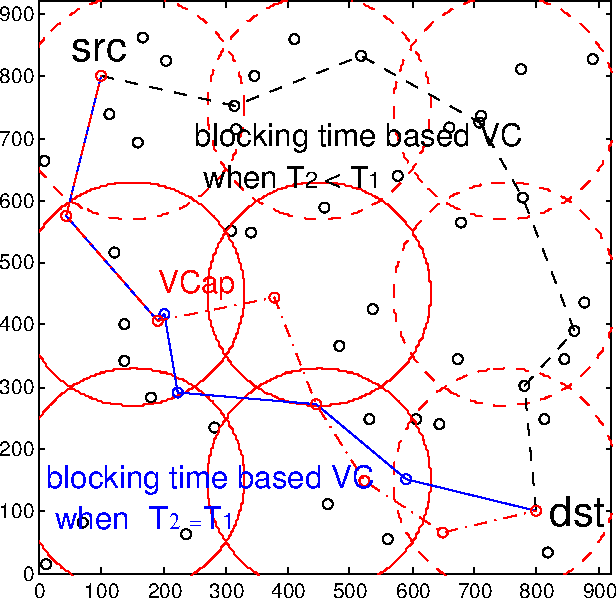
\includegraphics[width=0.6\linewidth]{topo_single_blocking_time.pdf}
    \caption{Routing paths in one network, $T_1 = 3s$. cycles denote the transmission range of primary uers.} 			\label{fig:multipleChannelPioff_case_topo}
\end{figure}
In the network, 9 primary users evenly distributed, $P_{\textsc{\tiny OFF}}=0.5$ for each of them.
For the primary users denoted by the solid cycles, maximal blocking time $T_1 = 3s$, and $T_2 = 1s$ and $3s$ for the other primary users.
When $T_2 < T_1$, the resultant routing path is in black and dashed, which goes through area where primary users have shorter maximal blocking time.
When $T_2 = T_1$, the resultant routing path largely converges with the path with VCap.

%and the $P_{\textsc{\tiny OFF}}$ of the other primary users changes from 0.5 yo 1, the PDR of the schemes is described in Figure~\ref{fig:fail_SA}.
%Note that although packet delivery ratio of SAViC increases when primary users become less intense, the packet loss of availability based virtual coordinate is only $10\%$ when there is $P_{\textsc{\tiny OFF}}=0.5$ for all primary.
%Due to the second available channel and the opportunistic spectrum access paradigm, the PDR of the three schemes are improved.
%%\vspace{.5cm}
%\begin{figure}[htb!]
%\subfigure[One CRN]{\label{fig:multipleChannelPioff_case_pdr}
%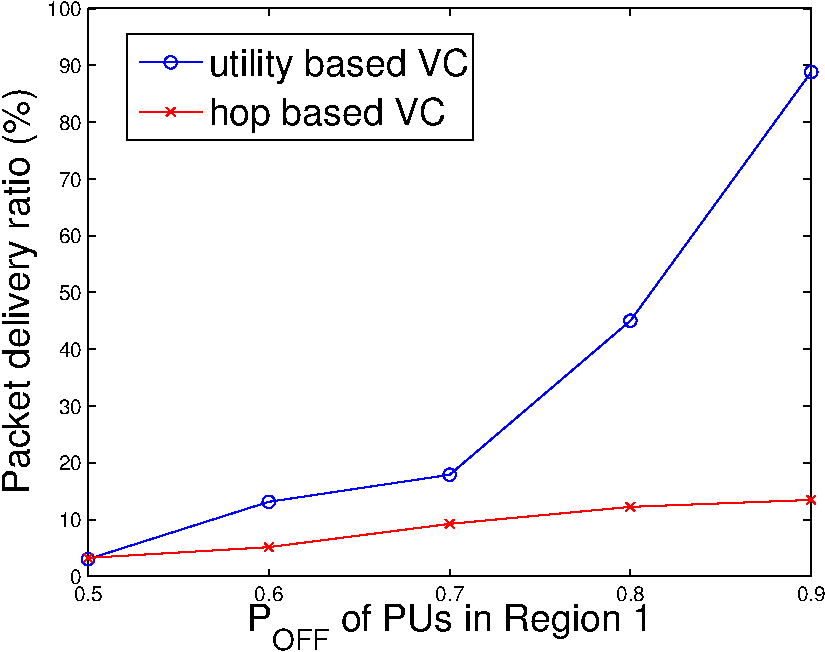
\includegraphics[width=0.455\linewidth]{MultiCH_DC_casestudy_pdr.pdf}
%}
%\subfigure[One CRN]{\label{fig:MultiChannel_DC_pdr}
%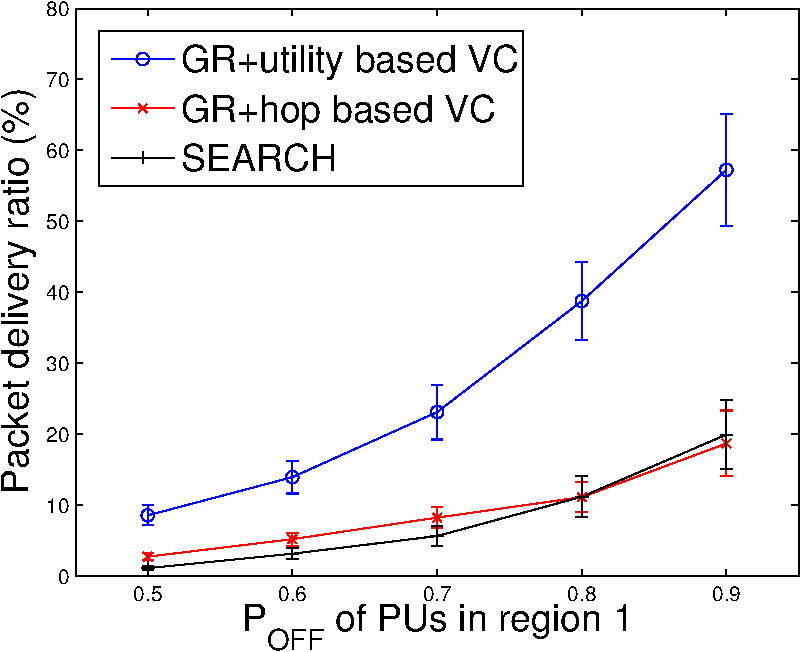
\includegraphics[width=0.455\linewidth]{multiCh_DC_average_pdr_3.pdf}
%}
%\label{fig:multiple_pioffCase}
%\caption{Packet delivery ratio in multiple secondary channel scenario}
%\end{figure}
%\vspace{.5cm}
%\begin{figure}[ht]
%	\centering
%    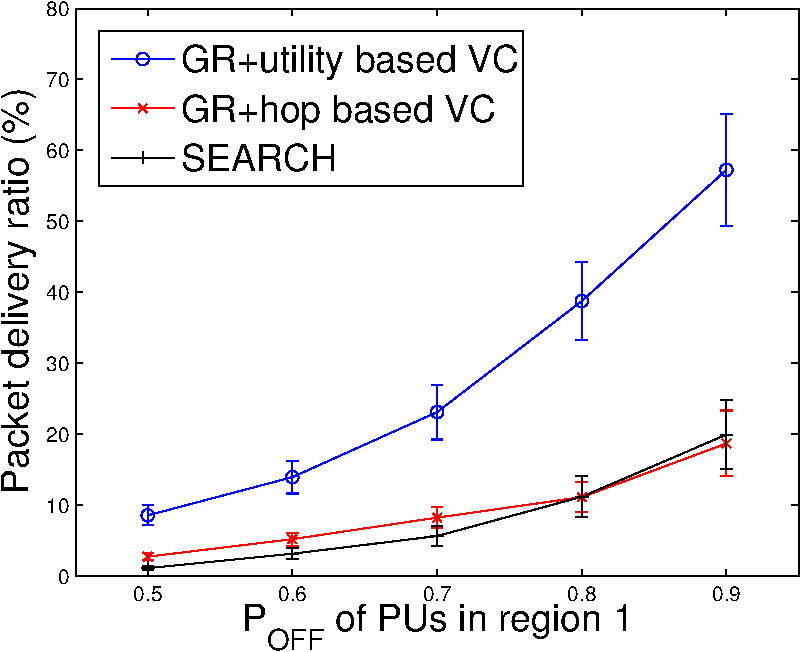
\includegraphics[width=0.6\linewidth]{multiCh_DC_average_pdr_3.pdf}
%    \caption{PDR of spectrum availability based virtual coordinate when likelihood is homogeneous in CRN} 			\label{fig:fail_SA}
%\end{figure}


The ineffectiveness of spectrum availability based virtual coordinate in case of identical $P_{\textsc{\tiny OFF}}$ is observed in Figure~\ref{fig:multipleChannelPioff_case_topo}.
In this case a different characteristic, i.e., the longest blocking time, which shows the geographically diverse characteristics of spectrum can be used.
In our simulation, $P_{\textsc{\tiny OFF}}=0.9$ for all primary users, but they are diverse on sojourn time, i.e. $T_1$ of primary user is 3s, and $T_2$ is shorter.
We randomize the location of secondary users in 50 networks, and present the performance of blocking time based virtual coordinate to show its superiority on decreased end to end delay and PDR.
In this part of simulation, we don't show the result of \textit{SEARCH}, as it performs as bad as geographic routing with hop based virtual coordinate.
The reason is the widespread primary users seriously hamper the routing requests to arrive at destination, consequentially most paths for forwarding the packets can not be constructed successfully.
\begin{figure}[htb!]
\subfigure[Packet delivery ratio]{\label{fig:SingleChannelEWT_randomness_rate}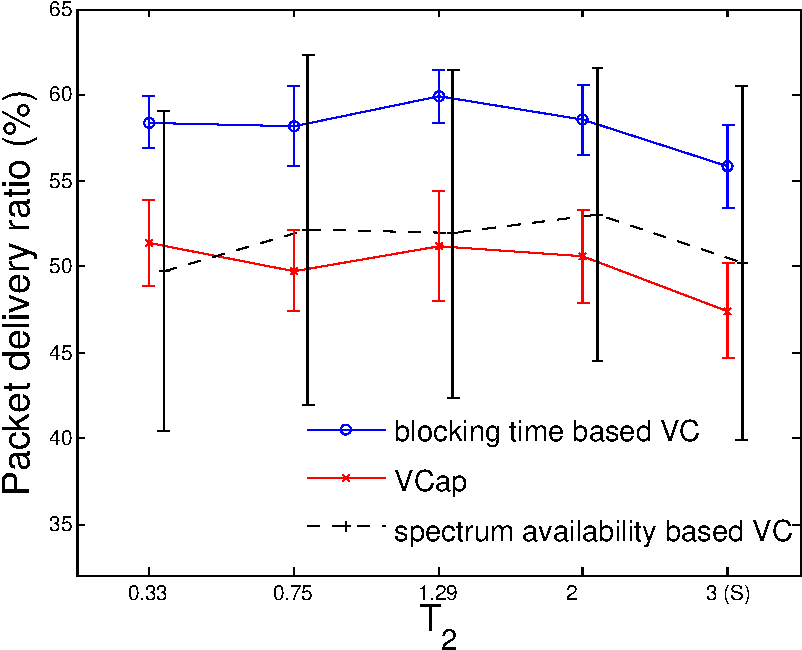
\includegraphics[width=0.46\linewidth]{ewt_pdr_3_ci.pdf}
}
\subfigure[Delay]{\label{fig:SingleChannelEWT_randomness_delay}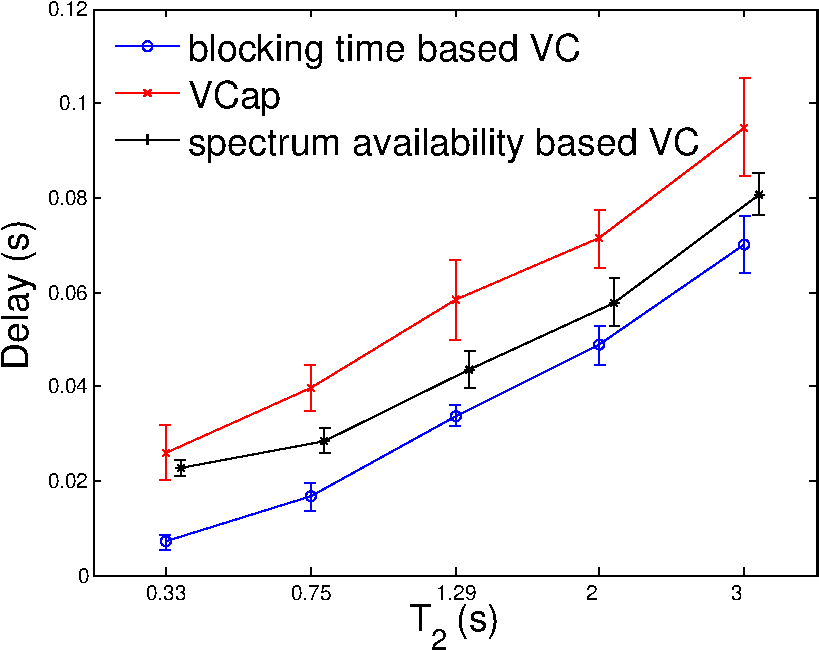
\includegraphics[width=0.46\linewidth]{delay_ewt_c1.pdf}
}
\label{fig:SingleChannelEWT}
\caption{Geographic routing in single secondary channel scenario, $P_{\textsc{\tiny OFF}}=0.9$ for all primary users, $T_1=3s$, $T_2$ varies.}
\end{figure}
%

%Because of \textit{SEARCH}'s weak performance when the whole network is influenced by primary users, (PDR is less 20\% as shown in Figure~\ref{fig:MultiChannel_DC_pdr}), we only compare the performances with delay based SAViC and hop based virtual coordinate.


Figure~\ref{fig:SingleChannelEWT_randomness_delay} shows as $T_2$ increases from 0.33s to 3s, the delay of successfully delivered packets also increases for both blocking time based virtual coordinate and VCap, but a constant gap exists in between.
Whereas, the delay of spectrum availability based virtual coordinate is random as respect to sojourn time, the reason is the routing metric in this scenario doesn't involve blocking time imposed by primary users.
%This shows blocking time based virtual coordinate enables routing path to go through primary user affecting areas where they have shorter sojourn time on operating.

%Delay based virtual coordinate manipulates nodes sharing smaller blocked time to get closer, whereas $P_{\textsc{\tiny OFF}}$ based virtual coordinate doesn't adjust the network topology meaningfully.

The packet delivery ratio shown in Figure \ref{fig:SingleChannelEWT_randomness_rate} is constant with both blocking time based virtual coordinate and VCap, because all the primary users have the same $P_{\textsc{\tiny OFF}}$ which is 0.9.
Particularly, blocking time based virtual coordinate achieves higher packet delivery ratio than the other two virtual ordinates, the reason is when the former is applied, less packets are dropped from buffer as the time of being blocked is shorter for the secondary users on the path.

%\vspace{.1cm}
%\textbf{Multiple secondary channel scenario}

%\textit{2. Multiple secondary channel scenario}





%The distinctive sojourn time of PUs in region 1 and 2 makes delay based virtual coordinate much effective to support geographic routing.
Now we have a look at the CRN with two licensed channels.
As to performance of delay, because of the second available channel, blocking time based virtual coordinate achieves very delay, in contrast, spectrum availability based virtual coordinate still demonstrates obvious randomness, as is shown in Figure \ref{fig:MultiChannelEWT_delay}. 
%Because of the second available channel, delay is primary user works on one more licensed channel and with the same pattern of the first channel.
Compare Figure \ref{fig:MultiChannelEWT_rate} and \ref{fig:SingleChannelEWT_randomness_rate}, we can see the packet delivery ratio in two channel network is obviously higher than that in single channel network, as the second channel provides extra transmission opportunities.
Blocking time based virtual coordinate achieves up to 10\% better performance than that with spectrum availability based VC, the reason is packets in buffer have greater likelihood to be sent out before getting dropped.
\begin{figure}[htb!]
\subfigure[Packet delivery ratio]{\label{fig:MultiChannelEWT_rate}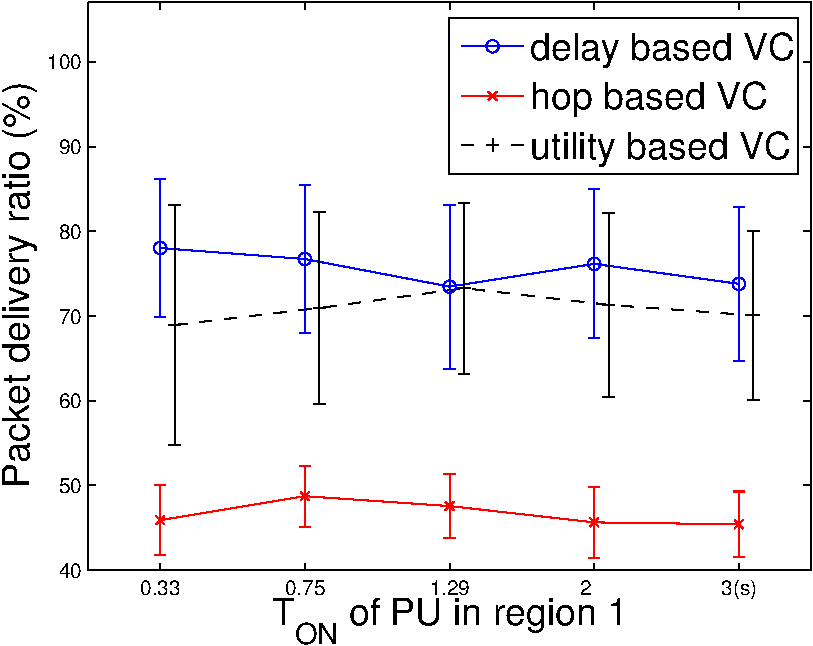
\includegraphics[width=0.46\linewidth]{multiCh_EWT_rate_3.pdf}
}
\subfigure[Delay]
{\label{fig:MultiChannelEWT_delay}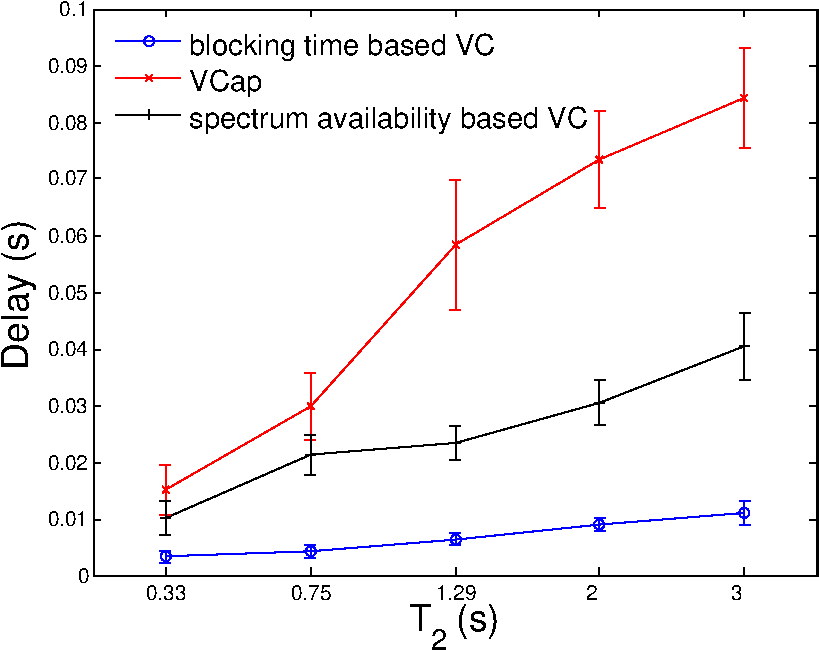
\includegraphics[width=0.46\linewidth]{delay_ewt_c2.pdf}
}
\label{fig:MultiChannelEWT_pdr}
\caption{Geographic routing in two secondary channel scenario, $P_{\textsc{\tiny OFF}}=0.9$ for all primary users, $T_1=3s$, $T_2$ varies.}
\end{figure}
%with each transition probability combination, we run the simulation in 10 randomly generated topologies (in each topology we measure the delay only once). The Results shown in Figure \ref{fig:SingleChannelEWT_diff_topos}, SA-VCap enabled path outperforms that from VCap in all criterions. The reason for low delivery ratio is that, PUs exist all over the network.

\subsection{Sensitivity of SAViC to Estimation Errors}
In this Section, we evaluate the performance of SAViC in the presence of erroneous estimates about the primary user activity.
In order to induce a particular amount of errors, we artificially add errors to duty cycle of primary user activity by directly modifying the implementation of 2 state markov chain. 
By doing this a real life scenario is built, where estimation errors are expected.
The simulation is conducted with the same configuration with Figure~\ref{fig:singleChannelPioff_case_topo}.
Figure~\ref{fig:errorenousEsti_DC} shows even the errors are significant, \ie DC is modified by 25\% to 100\%, the corresponding performance varies only at most 13\%.


\begin{figure}[ht]
	\centering
    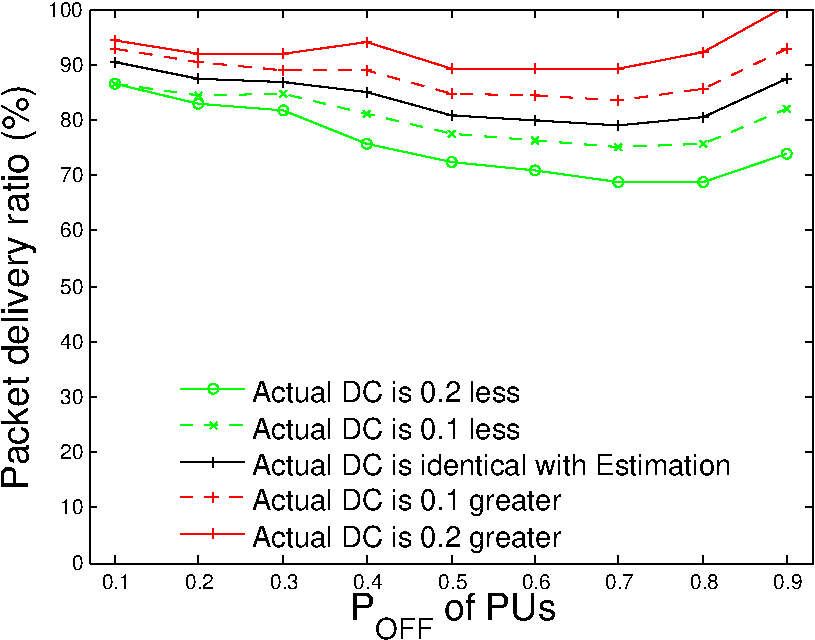
\includegraphics[width=0.7\linewidth]{errorenousEsti_DC.pdf}
    \caption{In the setting of Figure~\ref{fig:singleChannelPioff_case_topo}, perofrmance of DC based virtual coordinate is not affected greatly by the erroneous estimation} 			\label{fig:errorenousEsti_DC}
\end{figure}




\section{Conclusions}
The proposed virtual coordinate SAViC reshapes the topology of cognitive radio network based on sensing results of spectrum availability.
As SAViC adjusts the distance between nodes based on the communication obstruction caused by primary users, the virtual coordinate comprises a part of the routing decision, so that geographic routing is able to detour the areas seriously affected by primary user.
Geographic routing with SAViC greatly simplifies the computation and communication burden on each secondary user involved in routing in CRN.
Together with SAViC, geographic routing achieves better performances than other geographic routing designed for CRN through extensive simulation.
This paradigm of routing is especially suitable for CRN network where the resource limited CR nodes can only support geographic routing.
This work emphasises on avoiding primary users' influence with geographic routing, and doesn't consider the interference issue among the secondary users, which should be addressed in the future work.
%SAViC supports high reachability.
%As SAViC comprises routing decision, light weighted geographic routing circumvents the area seriously affected by primary user, or cut through the less affected area.
%Specially, geographic routing together with available channel likelihood based virtual coordinate achieve higher PDR than one representative CRN routing scheme when PUs' activities are geographically heterogeneous in the network.
%To remedy the incompetence of channel likelihood based VC, delay sensitive virtual coordinate becomes alternative to support geographic routing and produce short delay and satisfactory PDR.
%As a result, burden of computation and communication for secondary users is largely alleviated.
%The finally found path is static, which suffers from PUs' activity passively, a dynamic path adjustment scheme could be a workaround in the future work.
%\subsection{Choice on Characteristics of spectrum availability}
%The DT2MC provides a relatively comprehensive model to investigate PUs' activities.
%With the properties derived from DT2MC, we are able to design virtual coordinates emphasizing on different network performances.
%
%When primary users' characteristics are evenly distributed in the network, correspondingly designed virtual coordinate is not more effective than that based on hop number.